\documentclass{article}

\usepackage{graphicx}
\usepackage{placeins}
\usepackage[utf8]{inputenc}
\usepackage{listings}
\usepackage{hyperref}
\usepackage{xcolor}
\usepackage[nodayofweek,level]{datetime}
\usepackage{ulem}
\usepackage{mathtools}
\usepackage{newfloat}
\usepackage{seqsplit}

\usepackage{longtable}
\DeclareFloatingEnvironment[
    fileext=los,
    listname=List of code snippets,
    name=Snippet,
    placement=tbhp,
    within=none,
]{snippet}

\DeclarePairedDelimiter{\ceil}{\lceil}{\rceil}

\definecolor{darkgreen}{RGB}{0, 128, 0}
\definecolor{darkcyan}{RGB}{130, 230, 200}
\definecolor{verylightgray}{gray}{0.85}
\definecolor{goldenbrown}{rgb}{0.558215, 0.0, 0.135316}

\lstdefinelanguage{solidity}
{
	keywords={uint256, bytes32, mapping, address, uint40, bool, uint32, msg, sender, false, true},
	keywordstyle=\color{blue},
	keywords=[2]{pragma, contract, event, enum, struct, function, return, private, public, constant, returns, var, for, !, if, break, continue, throw, &&, ||, else, =, ==, <, >, <=, >=},
	keywordstyle=[2]\color{magenta},
	keywords=[3]{push, pull},	
	keywordstyle=[3]\color{darkcyan},
	comment=[l]{//},
	commentstyle=\color{darkgreen},
	numbers=left,
	extendedchars=false,
	morestring=[b]",
	stringstyle=\color{goldenbrown},
	breaklines=true,
	backgroundcolor=\color{verylightgray},
	basicstyle=\linespread{1}\ttfamily\footnotesize
}

\lstdefinelanguage{pseudocode}
{
	keywords={if, &&, true, false},
	keywordstyle=\color{blue},
	comment=[l]{//},
	commentstyle=\color{darkgreen}
}
\begin{document}

\normalem
\pagenumbering{Alph}
	\begin{titlepage}
		\noindent{\huge Consensus in declarative process models using distributed smart-contracts} \\ \\
		Mikkel Gaub, \\ Tróndur Høgnason, \\ Malthe Ettrup Kirkbro, \\ \& Mads Frederik Madsen	\\ \\
		\hspace{-18pt}
		\textit{May 15, 2017}
		\vspace{\fill}
		\section*{Abstract}
		This paper investigates how efficiently declarative process models can be implemented using distributed smart-contracts. 
		More concretely, a Dynamic Condition Response (DCR) workflow engine is implemented on the Ethereum platform, with a focus on minimizing the cost of running such an engine. 
		Two structurally different solutions are implemented and compared based on their cost.
		Then the best of the implementations is optimized, and a number of potential further features are described and their viability within the Ethereum platform are evaluated.
		\thispagestyle{empty}
	\end{titlepage}
	\clearpage

	\pagenumbering{arabic}
	\setcounter{page}{1}

	\setcounter{tocdepth}{2}
	\tableofcontents
	\pagebreak

	\section{Introduction}
	Coordinating a collaboration between several companies can be a daunting task.
	These collaborations can be complicated and time-sensitive.
	If the collaborations require some actions to be performed in a specific sequence, a workflow can be a used to describe this sequence.
	Ensuring agreement about the history of the workflow is pivotal.
	Consequently a single company cannot be in charge of administering the workflow, as they can only be trusted to act in their own interest, and forgery of the workflow history would be easy.
	Maintaining a valid history by preventing cheating while still giving all parties perfect information is therefore not a trivial task.

	We have previously explored the viability of solving these problems with blockchains in \cite{bachelor}, where we have shown how a blockchain can be used to achieve consensus between multiple participants in a declarative process model. 
	In this article we will continue to build upon our previous research with declarative process models on blockchain.

	As part of the research we built a proof of work declarative workflow management system (WfMS) that utilized Bitcoin's blockchain to achieve consensus. 
	We found Bitcoin's blockchain to be restrictive and expensive.
	This is primarily because Bitcoin's blockchain is not intended for anything else than a ledger of transactions for the cryptocurrency. 
	But the underlying technology, the blockchain, has been used in many other applications and platforms. 
	We will implement a WfMS using a Dynamic Condition Response (DCR) engine on one of these platforms, namely Ethereum -- which allows for storage of data and code execution on their blockchain.
	Since both code execution and storage costs money in Ethereum, optimization is key in order for a solution to be viable.
	Ethereum is also a very new technology and is constantly subject to change, making it fairly undocumented aside from the yellow paper \cite{yellow-paper} and white paper \cite{ethereum-white-paper}.
	We will therefore be experimenting with several different system structures and comparing their costs in order to find the best solution.

		\subsection{Previous work}
		Our previous work with blockchains was done for our bachelor thesis \cite{bachelor}. 
		The main idea we will carry on from our bachelor thesis is that a blockchain can be used to create a consensus protocol. 
		We will therefore not go into great detail of how we can achieve consensus with a blockchain. 
		The following section will provide the information we deem necessary to understand how we can achieve consensus with a blockchain, but no literature to support this. 
		Interested parties can review the previously mentioned thesis in which there is references to a great deal of literature to support this claim.

			\subsubsection{Achieving consensus with blockchains}
			In 2014 it was shown formally that Bitcoin's blockchain is a Monte Carlo solution to the Consensus Problem in a system with byzantine failures \cite{anonymous-byzantine-consensus}. 
			This proof is rather technical, and we will not go into further detail here.

			The consensus algorithms in Bitcoin and Ethereum are nearly identical, in that they are based on blockchains. It is therefore trivial to show that the same arguments presented for Bitcoin's consensus algorithm in \cite{anonymous-byzantine-consensus} holds for Ethereum.
			We have also given an argument for how the Bitcoin blockchain can be used to achieve consensus in a third party application in our bachelor's thesis. 
			For those interested in how consensus is ensured using blockchains, we suggest starting there.


			\subsubsection{Motivation to use Ethereum}
			The previous DCR engine we built utilized Bitcoins blockchain to validate workflow creation and execution attempts by storing the hash of these on the blockchain.
			The actual verification of the legality of executions with respect to DCR logic and execution rights was done on a DCR engine running locally on a users machine.
			Thus our application relied heavily on the majority of users involved in a workflow were actually using our DCR engine to verify the legality of executions. 

			Our previous DCR engine made it infeasible for an adversary to fake executions or claim that executions were part of another workflow than what benevolent users thought.
			Instead it was vulnerable to loss of local data. 
			
			If a user managed to remove all local traces of a workflow, it could be difficult to claim that the traces of executions belonged to a certain workflow and therefore hard to prove that a user actually did execute some specific activity. Furthermore reconstruction of a lost workflow would be nigh impossible without access to another copy of the workflow.

			Ethereums blockchain has other possibilities, as one is able to verify \textbf{1)} the existence of specific source code on the blockchain \textbf{2)} if code on the blockchain has been run \textbf{3)} if the code was run successfully or not.
			Any user participating in a workflow using a DCR engine running on Ethereums blockchain can therefore be sure\footnote{Quite sure...ref til vulnerabilities} that the source code is unchanged and that every execution is validated with respect to both DCR logic and execution rights in the same way Bitcoins blockchain verified workflow creation and execution attempts.

	\section{Dynamic Condition Response graphs}
	\label{sec:dcr-graphs}
	A DCR graph is a representation of a workflow.
	The graph is made up of one or more activities with a number of relations between them. 
	The following section is loosely based on a similar description in our bachelor's thesis \cite{bachelor}. 

		\subsection{Activity}
		The activities in a DCR graph have three attributes: included, executed and pending. 
		The attributes can be true or false. 
		Furthermore an activity can have role and actor specific execution rights.

			\subsubsection{Included attribute}
			If the include attribute of an activity is true, the activity is included and it can be executed. 
			If the attribute is false, the activity is excluded and can no longer be executed.

			\subsubsection{Pending attribute}
			If any activity in a workflow has a pending attribute that is true and the activity is included, the workflow is in an unfinished state.
			Every time an activity is executed its pending attribute is set to false.
			This means that setting the pending attribute of an included activity to true is specifying that this activity must be executed or excluded at some point to leave the workflow in a finished state.

			\subsubsection{Executed attribute}
			If an activities executed attribute is false executing the activity will set its executed attribute to true.
			Executing an already executed activity will have no effect on the executed attribute.

		\begin{figure}[!ht]
			\centering
			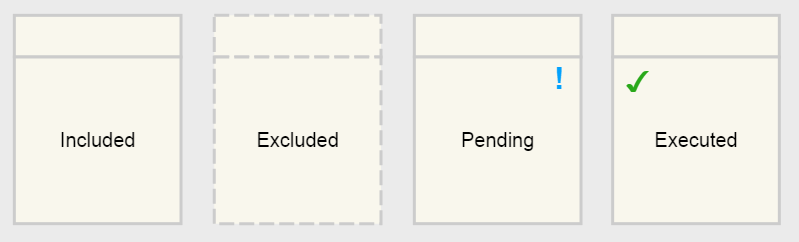
\includegraphics[width=1\textwidth]{figures/activity_states.png}
		 	\caption[Activity States]
		 	{From left to right: A visual representation of an included, excluded, pending and executed activity as presented on \href{http://www.dcrgraphs.net}{dcrgraphs.net}}.
		\end{figure}

		\subsection{Relations}
		There are five types of relations which define different types of relationships between activities in a workflow. 
		These five are the \emph{condition}, \emph{response}, \emph{include}, \emph{exclude} and \emph{milestone} relations.

			\subsubsection{Condition relation}
			If there is a condition relation from activity $A$ to activity $B$, then $B$ can only be executed if $A$'s executed attribute is true or $A$ is excluded.
			\begin{figure}[!ht]
				\centering
				
\includegraphics[width=0.3\textwidth]{figures/ConditionRelation.png}
			 	\caption[Condition relation]
			 	{Condition relation}
			\end{figure}

			\subsubsection{Response relation}
			If there is a response relation from activity $A$ to activity $B$, then $B$'s pending attribute will be set to true every time $A$ is executed.
			\begin{figure}[!ht]
				\centering
				
\includegraphics[width=0.3\textwidth]{figures/ResponseRelation.png}
			 	\caption[Response relation]
			 	{Response relation}
			\end{figure}

			\subsubsection{Include relation}
			If there is an include relation from activity $A$ to activity $B$, then $B$'s included attribute will be set to true every time $A$ is executed.
			\begin{figure}[!ht]
				\centering
				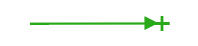
\includegraphics[width=0.3\textwidth]{figures/IncludeRelation.png}
			 	\caption[Include relation]
			 	{Include relation}
			\end{figure}

			\subsubsection{Exclude relation}
			If there is an exclude relation from activity $A$ to activity $B$, then $B$'s included attribute will be set to false every time $A$ is executed.
			\begin{figure}[!ht]
				\centering
				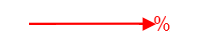
\includegraphics[width=0.3\textwidth]{figures/ExcludeRelation.png}
			 	\caption[Exclude relation]
			 	{Exclude relation}
			\end{figure}

			\subsubsection{Milestone relation}
			If there is a milestone relation from activity $A$ to activity $B$, then $B$ can only be executed if $A$'s pending attribute is false or $A$'s included attribute is false.
			\begin{figure}[!ht]
				\centering
				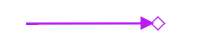
\includegraphics[width=0.3\textwidth]{figures/MilestoneRelation.png}
			 	\caption[Milestone relation]
			 	{Milestone relation}
			\end{figure}		

		\subsection{Example workflow}
		Figure \ref{fig:exampleWorkflow} shows a DCR graph modeling a support ticket workflow. When the workflow is created only \texttt{Submit ticket} is executable. 
		\texttt{Close ticket} cannot be executed as it is excluded and there is a condition relation to it from an unexecuted activity.
		The activities \texttt{Propose solution} and \texttt{Reject solution} cannot be executed as there are condition relations to them from activities that have not been executed. 
		Lastly \texttt{Accept solution} cannot be executed as there is a milestone relation to it from \texttt{Propose solution} which is pending and not excluded.

		\begin{figure}[!ht]
			\centering
			\includegraphics[width=\textwidth]{figures/exampleWorkflow.png}
		 	\caption[Example workflow]
		 	{Example workflow. Large version at appendix \ref{app:example-workflow}.}
		 	\label{fig:exampleWorkflow}
		\end{figure}
		\FloatBarrier

		A typical example of an execution order of the example workflow would look like this:
		\begin{enumerate}
			\item The customer executes \texttt{Submit ticket} which excludes itself. 
			This includes \texttt{Close ticket}, but \texttt{Close ticket} is still not executable, as there is a condition relation to it from \texttt{Accept solution}.
			\texttt{Propose solution} however is now executable.
			\item The supporter executes \texttt{Propose solution}. Now \texttt{Accept solution} is executable as \texttt{Propose solution} is no longer pending and \texttt{Reject solution} is also executable as \texttt{Propose solution} is executed. 
			Furthermore \texttt{Accept solution} is now pending and must therefore be executed or excluded at some point.
			\item If the customer is not satisfied with the solution he can execute \texttt{Reject solution} which will prevent execution of \texttt{Accept solution}, as \texttt{Propose solution} is now pending and still included. 
			The workflow is now in the same state as in step 2 except from the fact that \texttt{Reject solution} is executable. 
			Executing \texttt{Reject solution} will however have no effect, as \texttt{Propose solution} is already pending.
			\item If the customer on the other hand is satisfied with the supporters solution he can execute \texttt{Accept solution}.
			Executing \texttt{Accept solution} will exclude \texttt{Propose solution} and \texttt{Reject solution}.
			This leaves \texttt{Close ticket} executable and pending.
			To leave the workflow in a finished state the supporter must execute \texttt{Close ticket}. 
		\end{enumerate}

	\section{Ethereum}
		In order to implement the DCR engine as a distributed smart-contract, we use the platform Ethereum. 
		Ethereum is a blockchain technology that allows for code publication and execution via the Ethereum blockchain.  
		Central for blockchain technologies is a cryptocurrency, which is used to provide incentive for mining and to pay for the verification and computation of the published code.
		Ethereum's cryptocurrency is called \emph{Ether}.
		As an intermediary currency, the stack codes of the Ethereum Virtual Machine (EVM) have a value associated with it in a unit called gas, see appendix \ref{app:gas-prices}, which is then payed for with Ether by the person publishing that code.
		The EVM is, in the words of the creators of Ethereum, a "quasi-Turing-completeness"\cite{yellow-paper}.
		This is explained in that even if the gas is given away for free, there will be a structural limit in that unlimited gas is not representable.

		\subsection{Blockchain}
		\label{sec:blockchain}
		A blockchain is a distributed and decentralized database, consisting of blocks\cite{bitcoin-white-paper}. 
		Each block contains the changes to the database since the last block, as well as a reference to the block preceding it, thereby forming a chain.
		To ensure that data cannot be overwritten, each block must be verified by providing a solution to a cryptographic puzzle, namely finding a nonce, or proof-of-work, to include in the block such that the hash of the block information is below a variable threshold, called the difficulty\cite{bitcoin-white-paper}. 
		The process of finding a correct nonce is commonly called mining.
		The difficulty is automatically adjusted according to the frequency of mined blocks in relation to a desired frequency.
		Multiple blocks can be published simultaneously, and therefore reference the same preceding block. This situation is called a fork and is solved when one of the chains has a greater accumulated difficulty than the other.
		This typically means that the chain with the most blocks prevails, unless the network is partitioned unevenly and then reunited, as the difficulty within each partition will be automatically balanced to reflect the amount of computing power in that partition.

		The specifications of Ethereum's blockchain\cite{yellow-paper, ethereum-white-paper} contain some interesting features, which makes it different from most other blockchain technologies.
		
		Finding a proof-of-work in Bitcoin consists of incrementing the nonce and hashing the block header to check if it fulfills the difficulty requirements. 
		This is purely a question of computational power and has spawned a market for hardware specifically adapted to hashing, giving it an advantage compared to the standard processing units of a generic user. 
		As this hardware is fairly expensive, this favors the so called mining pools, which are large numbers of machines combining their computational power in order to find a proof-of-work and thereafter sharing the reward for mining a block. 
		This specialization undermines the decentralized aspect of the blockchain and in order to eliminate it, the proof-of-work in Ethereum is bound by memory.
		The bound by memory is implemented by using a hashing algorithm which involves creating a large directed graph and thereafter checking the values of a number of leaf-nodes as specified by an interpretation of the nonce. 
		The creators of Ethereum estimate that any significant progress in the performance of memory would be relatively cheap and widespread, as it is useful in many more situations than just in the mining of Ethereum blocks, as opposed to the hardware used for mining in Bitcoin.

		In Bitcoin, miners are rewarded by themselves when they mine the block, as they are allowed to include a transaction of a set amount of bitcoins to themselves.
		This is very similar to how Ethereum miners are rewarded, however they are additionally rewarded for including blocks that are not included in the longest chain.
		These are called uncles, or ommers, and are included in order to not have miners waste computational power, which would result in attackers potentially needing less than the majority of the network in order to overtake the currently longest chain, since Ethereum's blocks are mined much more frequently than Bitcoin's, which means that the speed of which blocks propagate becomes more pronounced. 
		The transactions contained in the uncles are ignored, as they could contain information conflicting with the contents of the blocks in the chain, but they are still included in the accumulated difficulty of the chain. Contrary to Bitcoins blockchain, where forks are resolved by choosing the longest chain, forks on Ethereums blockchain are solved by choosing the chain with the highest accumulated difficulty.
		Both the miners of the uncle and the miner who includes the uncle are rewarded in this system, with a fraction of the reward for mining a block contained in the main blockchain, ensuring incentive for miners to make the chain as heavy, difficulty-wise, as possible but still prioritizing mining new blocks.

		Aside from having to manage the balance of a users account, the blockchain of Ethereum also has the ability to store user-created code and arbitrary data encapsulated in so called smart-contracts (from hereon in called simply contracts). All users can interact with code on the blockchain, given that they can pay for the execution of said code. 
		When a transaction is included in a block, part of the verification of that block is running the code specified by the transaction and making sure that the state of the contract(s) affected by the transaction is mutated accordingly.

			\subsubsection{Data structure differences}
			Ethereum supports data storage and code execution, which has left the structure of its blockchain quite different from Bitcoin's.
			Firstly, Ethereum tracks the balance of each account as an unsigned integer, while Bitcoin accounts do not have an explicit balance, but rather uses unspent transactions, \emph{UTXO}'s, which are the transactions that have been sent to a specific account, but not yet been sent from that account. 
			This enables Bitcoin to track the origin of a single BTC all the way back to the minting of it.
			Since Ethereum has to support transactions which fail, but still cost Ether (see section \ref{sec:ethereum-virtual-machine}), they chose another solution better aligned with the rest of the platform.
			Rather than keeping track of unspent transactions in order to prevent the same money from being used twice, called double-spending, Ethereum maintains a counter for each contract, denoting how many times a transaction has originated from a given contract.

			\begin{figure}[!ht]
				\centering
				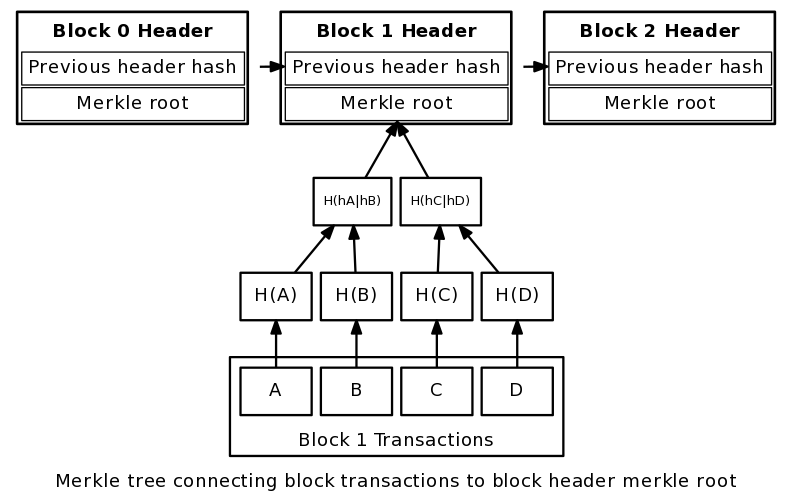
\includegraphics[scale=0.4, trim={0 1.2cm 0 0}, clip=true]{figures/merkle-tree.png}
			 	\caption[Bitcoin Merkle-tree]
			 	{Bitcoin Merkle-tree. Please note that the data contained in the block header is simplified. Borrowed from \url{https://yos.io/2016/05/19/merkle-trees-in-elixir/}}
			 	\label{fig:bitcoin-merkle-tree}
			\end{figure}

			Secondly, data and code must be stored somewhere, and verified on the blockchain.
			This is solved by making the contracts and accounts virtually the same element.  
			In Bitcoin, the integrity of accounts and transactions are verified by building a binary so-called \emph{Merkle-tree} of the transactions, and including the root of this tree in the block headers. 
			A Merkle-tree is a tree of hashes (see figure \ref{fig:bitcoin-merkle-tree}), such that the value of a parent, is its leaves concatenated and hashed. 
			This provides a way to verify if a transaction is in a block, by providing only $O(log(n))$ hashes, where $n$ is the number of transactions.
			It it also efficient to store in a block, since the root value can be used to verify the entire tree.
			By using UTXOs as currency tokens and Merkle-trees to verify transactions, Bitcoin sidesteps the issue of providing integrity for accounts; this is implied by the integrity of an account's transactions. 

			Ethereum, however, needs data- and code integrity as well, and thus cannot sidestep this issue.
			Due to the relatively low amount of time between block being mined in Ethereum and the fact that most of the contracts in the blockchain will be unaffected from block to block, Ethereum can optimize their space usage considerably if they can refer to subtrees in the previous block, rather than duplicating them, when nothing has changed in those subtrees. 
			To accomplish this, Ethereum uses a \emph{Merkle-Patricia tree} (also called Merkle-Patricia Trie). 

			\begin{figure}[!ht]
				\centering
				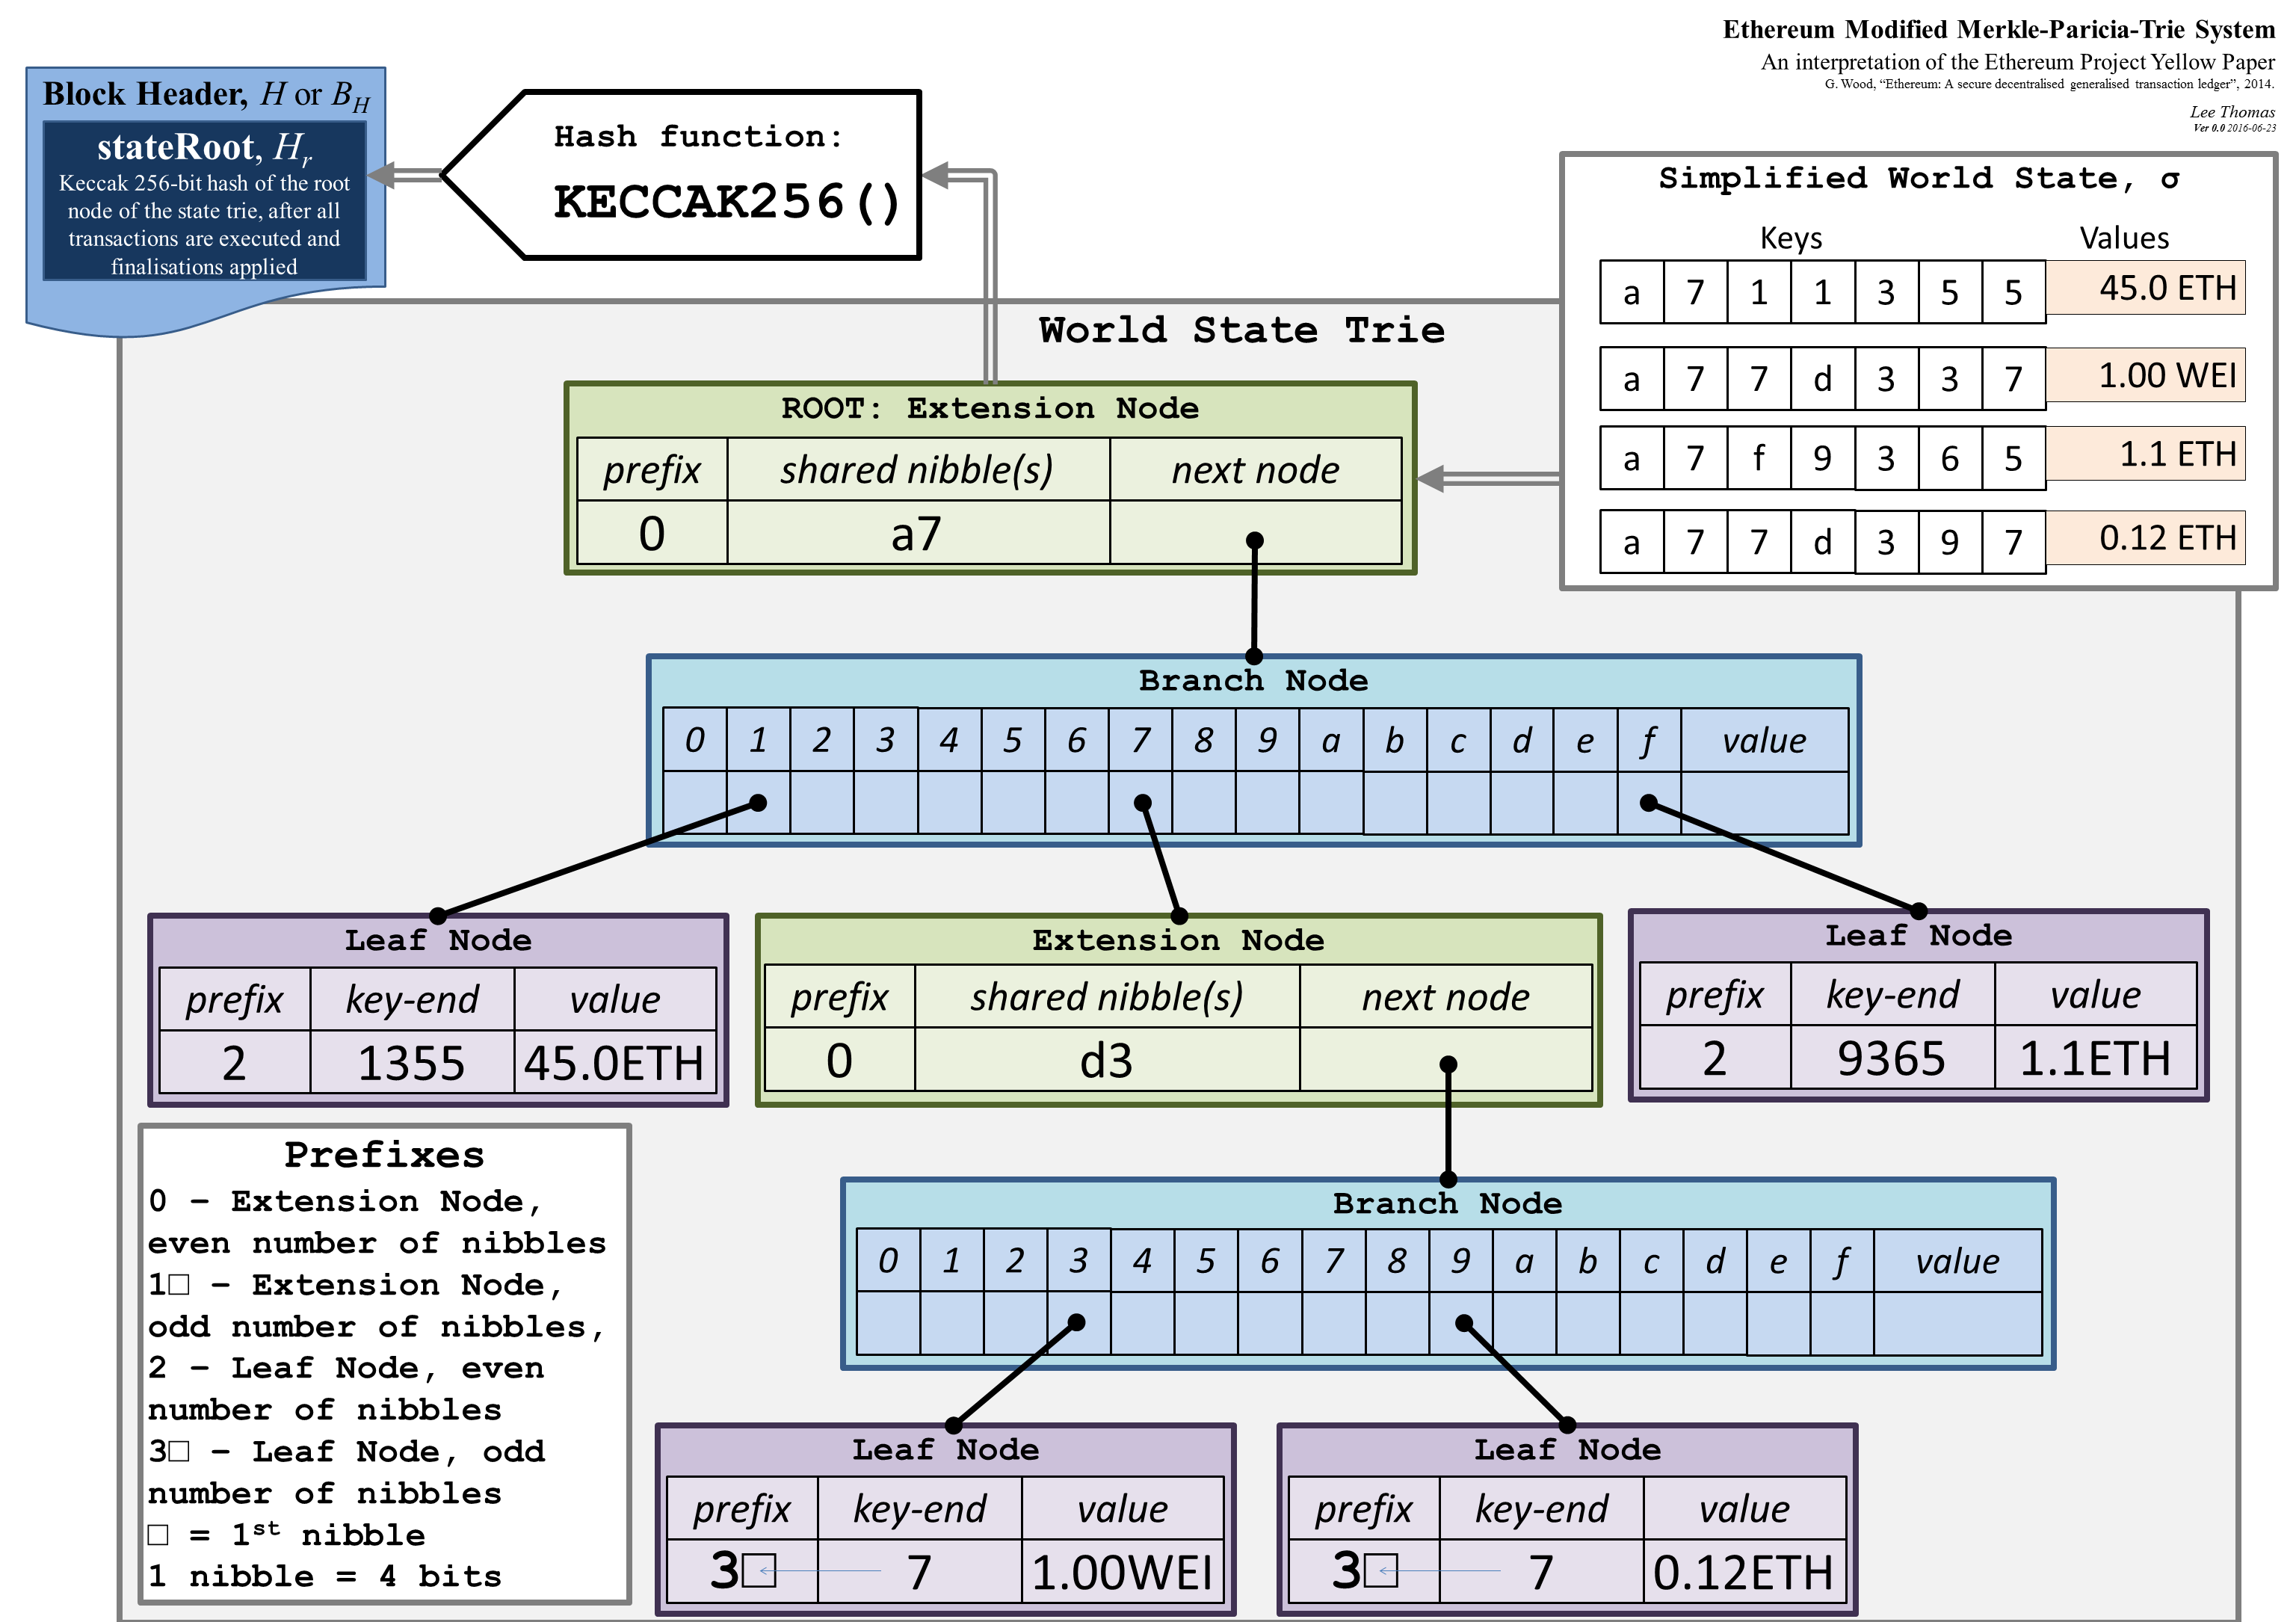
\includegraphics[scale=0.14]{figures/merkle-patricia-tree.png}
			 	\caption[Ethereum Merkle-Patricia tree example]
			 	{Ethereum Merkle-Patricia tree example, visualizing the basic data structure. Borrowed from \url{https://ethereum.stackexchange.com/questions/6415/eli5-how-does-a-merkle-patricia-trie-tree-work}}
			 	\label{fig:merkle-patricia-tree}
			\end{figure}

			The Merkle-Patricia trees differentiate themselves from the Merkle trees used by Bitcoin's blockchain, in the way that it is constructed.
			Each transactions placement in the Merkle-trees of Bitcoin are inconsequential, but is important in Ethereum because of its need for identifiable, and comparable, subtrees.
			The Merkle-Patricia tree is essentially a radix tree which uses hex representation of the keys, of the key-value pairs, as prefixes.
			As in figure \ref{fig:merkle-patricia-tree}, where all four accounts share the prefix \texttt{a7}, and thus are stored in the same extension node.
			The trie now branches the accounts out on three branches, according to their respective shared prefixes. 
			Since the accounts \texttt{a711355} and \texttt{a7f9365} do not share a prefix further than \texttt{a7} with other accounts, they are stored directly at this depth, thus saving unnecessary deepening of the tree.
			The fact that the Merkle-Patricia tree uses the account addresses (20 bytes) as prefixes, gives the tree a maximal depth of 40, and a branching factor of 16, making accesses to specific addresses very fast.  
			Finally, the are hashed together in manner specified by it being a Merkle-tree, making verification possible without having the entire tree, as in the Merkle-tree.  

			\begin{figure}[!ht]
				\centering
				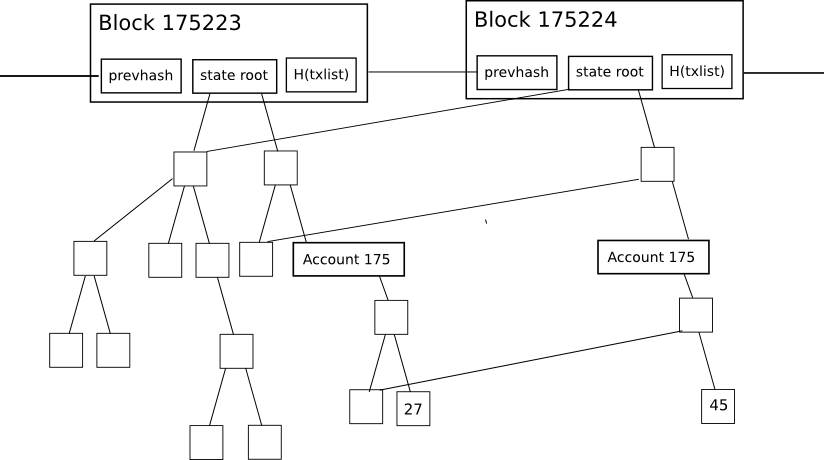
\includegraphics[scale=0.4]{figures/merkle-backref.png}
			 	\caption[Ethereum block header showing references to earlier blocks]
			 	{Ethereum block header showing references to earlier blocks' state-trees. Borrowed from \url{https://blog.ethereum.org/2015/06/26/state-tree-pruning/}}
			 	\label{fig:merkle-patricia-tree-references}
			\end{figure}

			When a change is made to an account, only the hashes along the branch containing the changed account needs to recomputed.

			These Merkle-Patricia trees are used for the receipts\footnote{These contain information such as gas used and which block the transaction was mined, and therefore verified, in} of the transactions, the state of each account after the transactions have been applied and the transactions themselves.

		\subsection{Currency}
		The distribution of Ether functions much like the distribution of bitcoins within the Bitcoin blockchain. 
		Mining a block has a base reward of five Ether, if it is included in the main blockchain.
		Ether is also earned in the creation of uncle blocks (See section \ref{sec:blockchain}).
		Lastly a miner also gets a reward based on how much computation power is needed to run the code included in a block. 
		The last reward is essentially equivalent to the transaction fees in Bitcoin.

		To store data or run code on the Ethereum platform one has to spend gas. 
		All computations have a set gas cost and can be seen in appendix \ref{app:gas-prices}, and Ethereum provides tools to estimate how much gas a proposed execution some code would cost.
		Gas has no inherent value, but instead a user has to specify how much Ether he wants to spend per gas. 
		The user then specifies how much gas he wants to send with the execution request and how much Ether he is willing to spend per gas. If the user has set the price he is willing to pay per gas too low, no miner will include the users code execution in his block.
		If on the other hand miners set their minimum price for inclusion too high, no one is willing to use Ethereum. 
		The price per gas is therefore based on the principle of supply and demand, where the commodity is computation power.

		If a user sends too little gas to complete the computations he requested, the requested computations are rolled back, but the user is still charged the spent gas.
		This is a security feature of Ethereum which prevents denial of service attacks by requesting many computationally heavy transactions without having the means to pay for them. 
		This feature is also what makes Ethereum quasi-Turing-complete rather than Turing-complete.

		\subsection{Ethereum Virtual Machine}	
		\label{sec:ethereum-virtual-machine}
		Due to the unique environment in which the EVM is used, there are equally unique constraints in the EVM:
		\begin{description}
			\item [Max stack size and limited stack access] The stack is limited to 1024 elements and COPY and SWAP operations can only access the top 16 elements of the stack. This infers some limitations on the number of parameters which can be given to a function.
			\item [No libraries] External functions are limited to what other contracts offer.  
			\item [No types] The EVM only operates in words of 32-byte Big Endian integers, meaning no floating point operations exist.
			\item [No true randoms] As part of block verification is ensuring that the state of a contract corresponds to the result of the functions performed on it, code needs to be deterministic and there are therefore no true random numbers.
			\item [Contract data access] All contracts are sandboxed inside their own environment, meaning that they cannot access the data of other contracts, except by calling their functions.
		\end{description}

		\subsubsection{Programming languages}
		There is a large number of options for programming languages which can compile to EVM bytecode, but due to Ethereum being a relatively new invention it is still subject to frequent low-level changes. 
		Most languages which can be compiled to EVM stack code are therefore languages specifically designed for Ethereum.
		Some of the languages implemented for Ethereum are Solidity, Viper, Serpent, LLL and Mutan which all are very basic at the moment, but the languages are all in active development, except for Mutan.

		We have chosen to implement our solutions in Solidity (v. 0.4.10) as it seems most mature of the listed options, at the time of writing.

		\subsection{Decentralized Applications}
		Since Ethereum is built around the concept of decentralized code execution, it enables what are called Decentralized Applications, or DApps. 
		A DApp is an application of which the back-end code is running on a decentralized peer-to-peer network, as for example on the Ethereum blockchain.
		The front-end can then be published on any or all of readily available platforms, such that anyone who is participating the peer-to-peer network can access it, achieving a fully decentralized application.


	\section{Implementation requirements}
	\label{sec:implementation-requirements}
	The data structure of the two implementation will be as follows:

	\begin{description}
		\item[Workflow] The workflow must contain a name, a list of activities and a list of access rights.
		\item[Activity] Each activity must contain a name, a list of the relations related to it and a list of users who are allowed to execute it.
		\item[Relations] The five relations described in Section \ref{sec:dcr-graphs} must be supported. They should be implemented in two categories:
			\begin{enumerate}
				\item Incoming: The relations in this category are the \emph{milestone} and \emph{condition}. These relations specify which other activities have \emph{milestone} or \emph{condition} relations to the activity containing the relations. Those activities' attributes must be checked to ensure the activity containing the relation can be executed.
				\item Outgoing: The relations in this category are the \emph{response}, \emph{exclude} and \emph{include} relation. These relations specify which activities' attributes must be updated after an execution on the activity containing the relation. 
			\end{enumerate}
		\item[Access rights] Should be indicated by the public key of a given user.
	\end{description}

	In order to ensure that the two implementations can be properly compared, they will support, and initially be limited to, the following functionality: 
	
	\begin{description}
		\item[Workflow creation] The implementations must support the creation of a workflow. Workflow creation should be performed with a single method call and must be atomic, meaning that no workflow can be partially created. This also means that no workflow can be modified past its creation.
		\item[Execution attempts] It must be possible to attempt to execute any activity at any time.
		\item[Activity execution] If an activity is executable following DCR logic, it must be executed if a user with the necessary rights requests an execution of it. The execution must also update the attributes of any other activities as prescribed by the outgoing relations it has.
		\item[Contract suicide] Any created contract must be allowed to self-destruct, when called by the creating user.
		\item[Data retrieval] The data stored must be accessible by any authorized user.
	\end{description}

	\section{Multi-contract implementation}

	The first implementation approach is to deploy an Ethereum contract for each workflow. We will call this implementation the Multi-contract implementation.
	Each deployed contract contains a workflows name, a list of the activities in the workflow and the address of the contract creator.
	Furthermore each contract contains functions to support the functionality described in section \ref{sec:implementation-requirements}.

	This approach ensures that only data relevant to the workflow, represented by the contract, is stored on the contract. The Multi-contract implementation therefore achieves a relatively high level of cohesion.
	Another approach could be to deploy each activity as its own contract.
	However this approach would introduce a high level of coupling between contracts.
	The Multi-contract implementation on the other hand achieves minimum coupling between contracts, since no inter-contract function calls are necessary to achieve the required functionality.

	% Important implementation details
		%Data structure
		\subsection{Implementation details}
		The data structures in the Multi-contract implementation are relatively simple.
		Only a single struct is defined, which represents an activity.
		The entire contract is the workflow, so no explicit data structure is need for the workflow. 
		Instead the contract's fields contain the relevant data for the workflow.
		The contract contains a \texttt{bytes32 name} field representing the workflows name, an array of activities and the Ethereum address of the creator of the workflow.
		\begin{snippet}[!ht]
			\centering
			\begin{lstlisting}[language=solidity, numbers=none]
struct Activity {
    // State
    bytes32 name;
    bool included;
    bool executed;
    bool pending;

    // Outgoing relations:
    uint32[] include;
    uint32[] exclude;
    uint32[] response;
    
    // Incoming relations:
    uint32[] condition;
    uint32[] milestone;

    // Access rights:
    address[] whitelist;
}				
			\end{lstlisting}
		 	\caption[The \texttt{Activity} struct]
		 	{The \texttt{Activity} struct}
		 	\label{sni:activity-struct}
		\end{snippet}
		The \texttt{Activity} struct shown in snippet \ref{sni:activity-struct} is made up of a \texttt{bytes32} name, three boolean values representing an activity's attributes, an array for each relation type and a list of Ethereum addresses that are authorized to execute the activity.

		%Construction
		The entire workflow is initialized when the contract is deployed.
		Since the Solidity language currently does not support neither structs nor nested arrays as parameters in contract deployment, the workflow initialization is a bit complicated. 

		For instance, every relation in the workflow is represented in a single \texttt{uint32} list in the constructor, called \texttt{relations}. 
		To map the relations to activities (see snippet \ref{sni:relation-mapping}), the structure of the relations-array has to uphold the invariant that, for an even \texttt{i}, \texttt{relations[i]} is the id of the activity the relation is coming from, and \texttt{relations[i+1]} is the id of the activity the relation pointing to.

		Excluding contract construction, the rest of the functions are reasonably simple.
		The code for the Multi-contract implementation can be found in its entirety in appendix \ref{app:multi-contract-code}.

		\begin{snippet}[!ht]
			\centering
			\begin{lstlisting}[language=solidity, numbers=none]
// We expect the 'relations' array is formed such that the first index is the FROM activity and the next index is the TO activity. Rinse and repeat.
for(i = 0; i < relations.length; i=i+2){
    if(relationType[i/2] == RelationType.Include)        	activities[relations[i]].include.push(relations[i+1]);
    else if(relationType[i/2] == RelationType.Exclude)   	activities[relations[i]].exclude.push(relations[i+1]);
    else if(relationType[i/2] == RelationType.Response)  	activities[relations[i]].response.push(relations[i+1]);
    else if(relationType[i/2] == RelationType.Condition) 	activities[relations[i+1]].condition.push(relations[i]);
    else if(relationType[i/2] == RelationType.Milestone) 	activities[relations[i+1]].milestone.push(relations[i]);
    else throw;
}			
			\end{lstlisting}
		 	\caption[Mapping relations to activities in the multi-contract construction]
		 	{Mapping relations to activities in the multi-contract construction}
		 	\label{sni:relation-mapping}
		\end{snippet}
	% How it runs missing

	\section{Mono-contract implementation}
	The idea behind the second implementation is that the gas costs of Ethereum are largely dominated by the price of creating a contract. If we observe appendix \ref{app:gas-prices} we find that the most expensive operation is the contract creation operation $G_{create}$ which costs 32000 gas. 
	This incentiveses us to create as few contracts as possible. 

	The second implementation is therefore a single contract with all workflows. 
	Workflows that are created are stored in a workflow array. 
	The methods of the Mono-contract implementation are largely the same as in the Multi-contract implementation. 
	The key difference is that the methods must access an index of the workflow array to retrieve the specified array before beginning modification of a workflow.

	The limitations of Solidity are clearly reflected in the \texttt{createWorkflow} method which creates a workflow. 
	Because of the limit on number of bytes the EVM can go back on the stack, the number of variables a method can take is limited. 
	This limitation creates problems for methods which require large amount of different data. 
	Some of the compromises we have made to limit the number of variables in the \texttt{createWorkflow} are listed below:
	\begin{enumerate}
		\item A byte array is used to represent all names relevant to the workflow. The first index is used for the workflow name, indices 1 to $n$ (where $n$ is the number of activities minus 31) are used for activity names.
		\item Instead of three boolean lists representing the attributes of the activities, the array \texttt{activityStates} contains the three boolean lists.
		\item An array of size three of unsigned integer arrays is used to represent activity data. 
		\begin{enumerate}
			\item The first array is used as a counter for how many relations will be stored on each activity. We use this counter as there is only one array containing the type of the relation and one array containing the id of the activity the relation should point to. But there is nothing indicating which activity the relation should be stored on.
			\item The second array is used to represent the number of public keys that are authorized to execute an activity. This counter is used as there is only a single list with all authorized user, but there is nothing associating them with any specific activity.
		\end{enumerate}
	\end{enumerate}

	\section{Comparison}
	\label{sec:comparison}

	In order to compare the implementations we have created an example workflow, see figure \ref{fig:exampleWorkflow}, on which we will execute activities in a specific order. Some of the executions should fail, as the executions are also used to test if the DCR logic is implemented correctly(See appendix \ref{app:test-cases-gas}).
	Due to the nature of our implementations, we anticipate that the act of creating the contract and subsequently the workflow will be the most expensive operation, by a large margin.

	In the Multi-contract implementation the cost of creating a workflow is included in the cost of deploying the contract, while these two costs are separate in the Mono-contract implementation.
	This difference complicates the comparison of the two implementation.

	Appendix \ref{app:test-cases-gas} shows that the cost of creating a contract containing the example workflow in the Multi-contract implementation costs $2,221,906$ gas.
	In the Mono-contract implementation, the equivalent operation cost 

	$$2,183,805\quad(contract) + 1,010,934\quad(workflow) = 3,194,739$$

	\noindent gas. These results give us the impression that the Multi-contract implementation might be the superior implementation in terms of gas cost
	However, the point of the Mono-contract implementation is to minimize the cost of creating workflows after contract creation, since only one contract creations is required. 

	Table \ref{tab:cost-of-creating-multiple-workflows} shows that already after the second workflow creation, 253,139 gas has been saved by using the Mono-contract implementation.
	Our assumption that the Mono-implementation is more cost-effective in the long run, therefore seems to hold.  

	\begin{table}[]
		\centering
		\label{tab:cost-of-creating-multiple-workflows}
		\begin{tabular}{|p{2.5cm}|p{2.5cm}|p{2.5cm}|p{2.5cm}|}
			\hline
			Number of workflows & Multi-contract cost (gas) & Mono-contract cost (gas) 	& Difference (Multi $-$ Mono)   \\\hline
			1                   & 2,221,906                 & 3,194,739                 & -972,833          			\\\hline
			2                   & 4,443,812                 & 4,190,673                 & 253,139          				\\\hline
			3                   & 6,665,718                 & 5,186,607                 & 1,479,111          			\\\hline
			4                   & 8,887,624                 & 6,182,541                 & 2,705,083          			\\\hline
			5                   & 11,109,530                & 7,178,475                 & 3,931,055          			\\\hline
			6                   & 13,331,436                & 8,174,409                 & 5,157,027          			\\\hline
			7                   & 15,553,342                & 9,170,343                 & 6,382,999          			\\\hline
			8                   & 17,775,248                & 10,166,277                & 7,608,971          			\\\hline
			9                   & 19,997,154                & 11,162,211                & 8,834,943          			\\\hline
			10                  & 22,219,060                & 12,158,145                & 10,060,915          			\\\hline
		\end{tabular}      
		\caption{Gas cost of creating multiple instances of the example workflow, and the difference between implementations}
	\end{table}

	Interestingly it can also be observed in appendix \ref{app:test-cases-gas} that the second and third creation of the example workflow in the Mono-contract implementation are cheaper than the first creation of the example workflow.

	We expect this is due to the fact that the array holding the workflows must be initialized on creation of the first workflow.
	Subsequent creations of the example workflow cost $995,934$ gas, a difference of $1,010,934 - 995,934 = 15,000$ gas.	

	The cost of executing activities is however cheaper in the Multi-contract implementation as seen in table \ref{tab:cost-of-executing-activities}.
	We expect this is due to the fact that there are more list look-ups in the Mono-contract implementation, since there is a need to first load the workflow, and then the activity.

	The cost of executing an activity is also affected by how many relations are stored on it. 
	Table \ref{tab:cost-of-executing-activities} clearly shows that executing \texttt{Reject solution}, which has two relations stored on it, is cheaper than executing \texttt{Submit ticket}, which has three relations stored on it.
	It can also be observed in table \ref{tab:cost-of-executing-activities} that the difference of the cost of executing an activity in the two implementations grows, if more relations are stored on the executed activity.
	Since each relation is a lookup or change of another activity's attributes, the growing difference in execution cost in our implementations supports our hypothesis that the increased cost of execution in the Mono-contract implementation is due to look-up of both workflow and activity.

	\begin{table}[!ht]
		\centering
		\label{tab:cost-of-executing-activities}
		\begin{tabular}{|p{3cm}|p{2.5cm}|p{2.5cm}|p{2.5cm}|}
			\hline
			Activity                     & Multi-contract cost (gas) & Mono-contract cost (gas) & Difference (Mono $-$ Multi) \\\hline
			Submit ticket                & 61,112          			 & 61,187         			& 75         \\\hline
			Propose solution             & 41,208          			 & 41,263         			& 55         \\\hline
			Reject solution              & 41,208          			 & 41,263         			& 55         \\\hline
			Propose solution             & 41,208          			 & 41,263         			& 55         \\\hline
			Accept solution              & 54,023          			 & 54,118         			& 95         \\\hline
			Close ticket                 & 34,810          			 & 34,845         			& 35         \\\hline
		\end{tabular}
		\caption{Gas cost of executing activities in the example workflow, and the difference between implementations}
	\end{table}

	We consider the large winnings in workflow creations to more than make up for cost increase in activity execution, and will continue to optimize on the Mono-contract implementation.

		 

	% Additionally we have also created tests for edge cases, where two activities are connected by a single relation.
	% This is done for each relation in order to get an estimate for the cost of a single such operation.
	% Stress tests are also performed for a reasonable number of each activities, in order to test for unforeseen sudden cost increases for any of the relations.


	\section{Optimizations}
		Using the results from section \ref{sec:comparison}, we optimized the mono-contract implementation, with the goal of reducing the cost usage even further.
		We have prioritized the optimizations according to an idea of the frequency of use, meaning that for example the mono-contract solution is based on the assumption that workflow creation is much more frequent than contract creation.
		Therefore a cost decrease of the workflow creation functionality is acceptable even if at the cost of making contract creation more expensive. 
		Similarly, optimizations with regards to the cost of activity executions at the expense of workflow creation is desirable.

		\subsection{Bitvectors}
		In the previous section we saw that cost of executing an activity is largely influenced by the number relations it has -- how many lookups or changes in other activities' attributes are needed.

		Since the number of relation an activity has is 

		In order to  cost of activity executions, we have implemented the activities as bitvector fields. 
		That is, we have removed the activity struct entirely, and instead put the state- and relation data into \texttt{uint256} types and store them in the workflow struct (see snippet \ref{sni:bitvectors}).
		
		\begin{snippet}[ht!]
			\centering
			\lstinputlisting[language=solidity, firstline=11, lastline=30, numbers=none]{../contracts/optimizations/monolith-bitvectors.sol}
		 	\caption[Activities as bitvectors]
		 	{Activities as bitvectors}
		 	\label{sni:bitvectors}
		\end{snippet}

		This change naturally has several effects.
		As a negative consequence, this limits the number of activities a workflow can contain to 256, since each bit of the three \emph{uint256} represents one of an activity's three attributes.
		However we do not expect workflows with more than 256 activities to be a normal occurrence.
		If the need for workflows of a greater size arises, we suggest the need could be addressed by partitioning the the workflow into 256-activity sized sub-workflows, and connecting the two workflows using external relations (see section \ref{sec:external-relations} for an in-depth explanation of external relations).

		We expected workflow creation to become costlier as at trade-off for cheaper activity executions, however this was not the case. Table \ref{table:test-cases-bitvectors} shows a comparison of the costs of creating the example workflow and executing its activities in the Mono-contract implementation and the Mono-contract-bitvector implementation.
		Surprisingly the creation of the example workflow was cheaper in the Mono-contract-bitvector implementation, and executions were generally more expensive.

		\begin{tabular}{| l | l | l |}
		\label{table:test-cases-bitvectors}
			\hline
			Action 							& Mono-contract  & Mono-contract with bitvectors \\ \hline
			1. Contract creation			& 2183805		 & 1708991 	\\\hline
			2. Workflow creation (1)		& 1010934 		 & 835045 	\\\hline
			3. Submit ticket				& 61187			 & 66591	\\\hline
			4. Propose solution				& 41263 		 & 51805	\\\hline
			5. Propose solution (Duplicate)	& 41263 		 & 51805	\\\hline
			6. Reject solution				& 41263 		 & 51805	\\\hline
			7. Propose solution				& 41263 		 & 51805	\\\hline
			8. Accept solution				& 54118 		 & 51805	\\\hline
			9. Close ticket					& 34845 		 & 36805	\\\hline
			10.Workflow creation (2)		& 995934 		 & 820045	\\\hline
			11.Workflow creation (3)		& 995934 		 & 820045	\\\hline
			\hline
		\end{tabular}
		\pagebreak


		Secondly, since each relation-type (i.e. Condition, Include, etc.) is represented as an \texttt{uint256} per activity, the creation of a workflow will usually be more expensive, unless the workflow is unusually relation-dense. 
		This is due to the fact that we allocate 5 bitvectors (one per relation type) of size 256, per activity. 
		Excluding the overhead of the lists holding the bitvectors, the storage space required for relations after the optimization can be expressed as $s = 5 \cdot 256 \cdot a$, where $a$ is the number of activities, and $s$ it the storage required in bits.
		Before the optimization, the relations were represented by a single \texttt{uint32} per relation.
		So the storage requirements before the optimization, excluding any overhead on the lists holding the relations, can be expressed as $s = 32 \cdot r$, where $r$ is the number of relations.
		Thus, for the bitvector optimization to be an optimization with regards to storage, there have to be more than 40 times as many relations as activities:

		\begin{center}		
			$32 \cdot r = 5 \cdot 256 \cdot a \iff r = \frac{1280 \cdot a}{32} \iff \frac{r}{a} = 40$
		\end{center}
		
		While this will rarely be the case, we still view this as an acceptable optimization if there is a noticeable gain on the activity execution.

		\subsection{Call data}
		% While the bitvector implementation might not be an optimization for activity execution, it comes at the cost of workflow creation. 
		% However, there is a hidden optimization opportunity, gained by implementing the activities as bitvectors. 
		For comparison purposes we have kept the \texttt{createWorkflow} parameters as close to the original Mono-contract implementation as possible. 
		But since the parameters have to be kept in the transaction, the call data actually uses storage space and so costs gas.
		So by reducing the amount of data being sent, we can make the creation of a workflow cheaper, which the bitvector implementation has enabled to higher degree. 
		Furthermore, since we are not making structs any more, we can, with a few exceptions, send the raw data to be stored, thus saving conversion operations. 

	\section{Discussion}

	\section{GUI}

	\section{Further features}
	As the optimized solution is a completely bare-bones implementation of a DCR engine, there are multiple potential expansions of the functionality and features which could be implemented on top of the current structure, both with regards to the functionality supported by DCR and by Ethereum.
	These features would be fairly use-case dependent and since they would have an effect on the cost of running a workflow, they should only be implemented in instances where they would actually be used.

		\subsection{Workflow changes}
		\label{sec:workflow-changes}

		In the case where a companies definition of a workflow changes, but the workflow models an ongoing process, it would be beneficial to simply change the workflow according to the specifications of the new workflow.
		This poses some challenges in the way that the workflow might change its definition, subtly or drastically, as covered in \cite{hierarchical-declarative-modelling} with regards to refinement.
		
		Implementing an algorithm that could verify that any given change to a workflow does not make the workflow less restrictive and deploying it on Ethereum's blockchain would be possible.
		However this is a computationally hard problem and therefore expensive to run on Ethereum.\footnote{Nok en ref på at det er svært}

			\subsubsection{Vulnerabilities}
			Allowing dynamic changes to workflows does not directly introduce any vulnerabilities. 
			However different implementations of this feature can lead to rising activity execution costs, unfairness and lessens the trust in the system. 
			Care must therefore be taken to ensure everyone involved in the workflow understands the implications of allowing dynamic changes.

			Firstly adding an activity $A$ with 1000 condition relations to another activity $B$ would greatly increase the cost of running $B$\footnote{This is only possible in the unoptimized implementations. However a case of adding 1000 activities $\{A_1, A_2, \dots, A_{1000}\}$, each with a condition to $B$ would have the same effect.}, as an execution of $B$ would result in checking a 1000 times if $A$ was executed or excluded. 

			Secondly changing a workflow could make it less restrictive. 
			This is true when the added activities have include or exclude relations to existing activities in the workflow \cite{dynamic-workflows}.

			Thirdly while only allowing activities with condition, response and milestone relations to other activities to be added to the workflow after creation, would only make the workflow more restrictive, a workflow could enter a deadlock where no activity could be executed.

			A middle ground could be reached by implementing dynamic changes to workflows as staged changes, and then to allow affected parties to vote on whether or not the changes should be allowed.
			Solidity supports implementing this kind of voting on Ethereum's blockchain.\cite{voting} 
			If dynamic changes should be allowed, which changes should be allowed and who should be allowed to perform them is subject to interpretation, and is based on the use case of each single workflow.

		\subsection{External relations}
		\label{sec:external-relations}
		In the proposed solutions, workflows are viewed as completely separate from each other. 
		This means that if a relation between the two is desired, it would require the entire workflow to be duplicated per other workflow relevant to it.
		An alternative to this, could be to create external relations between the workflows, as described in \cite{distributed-workflows}.

		\begin{figure}[!ht]
			\centering
			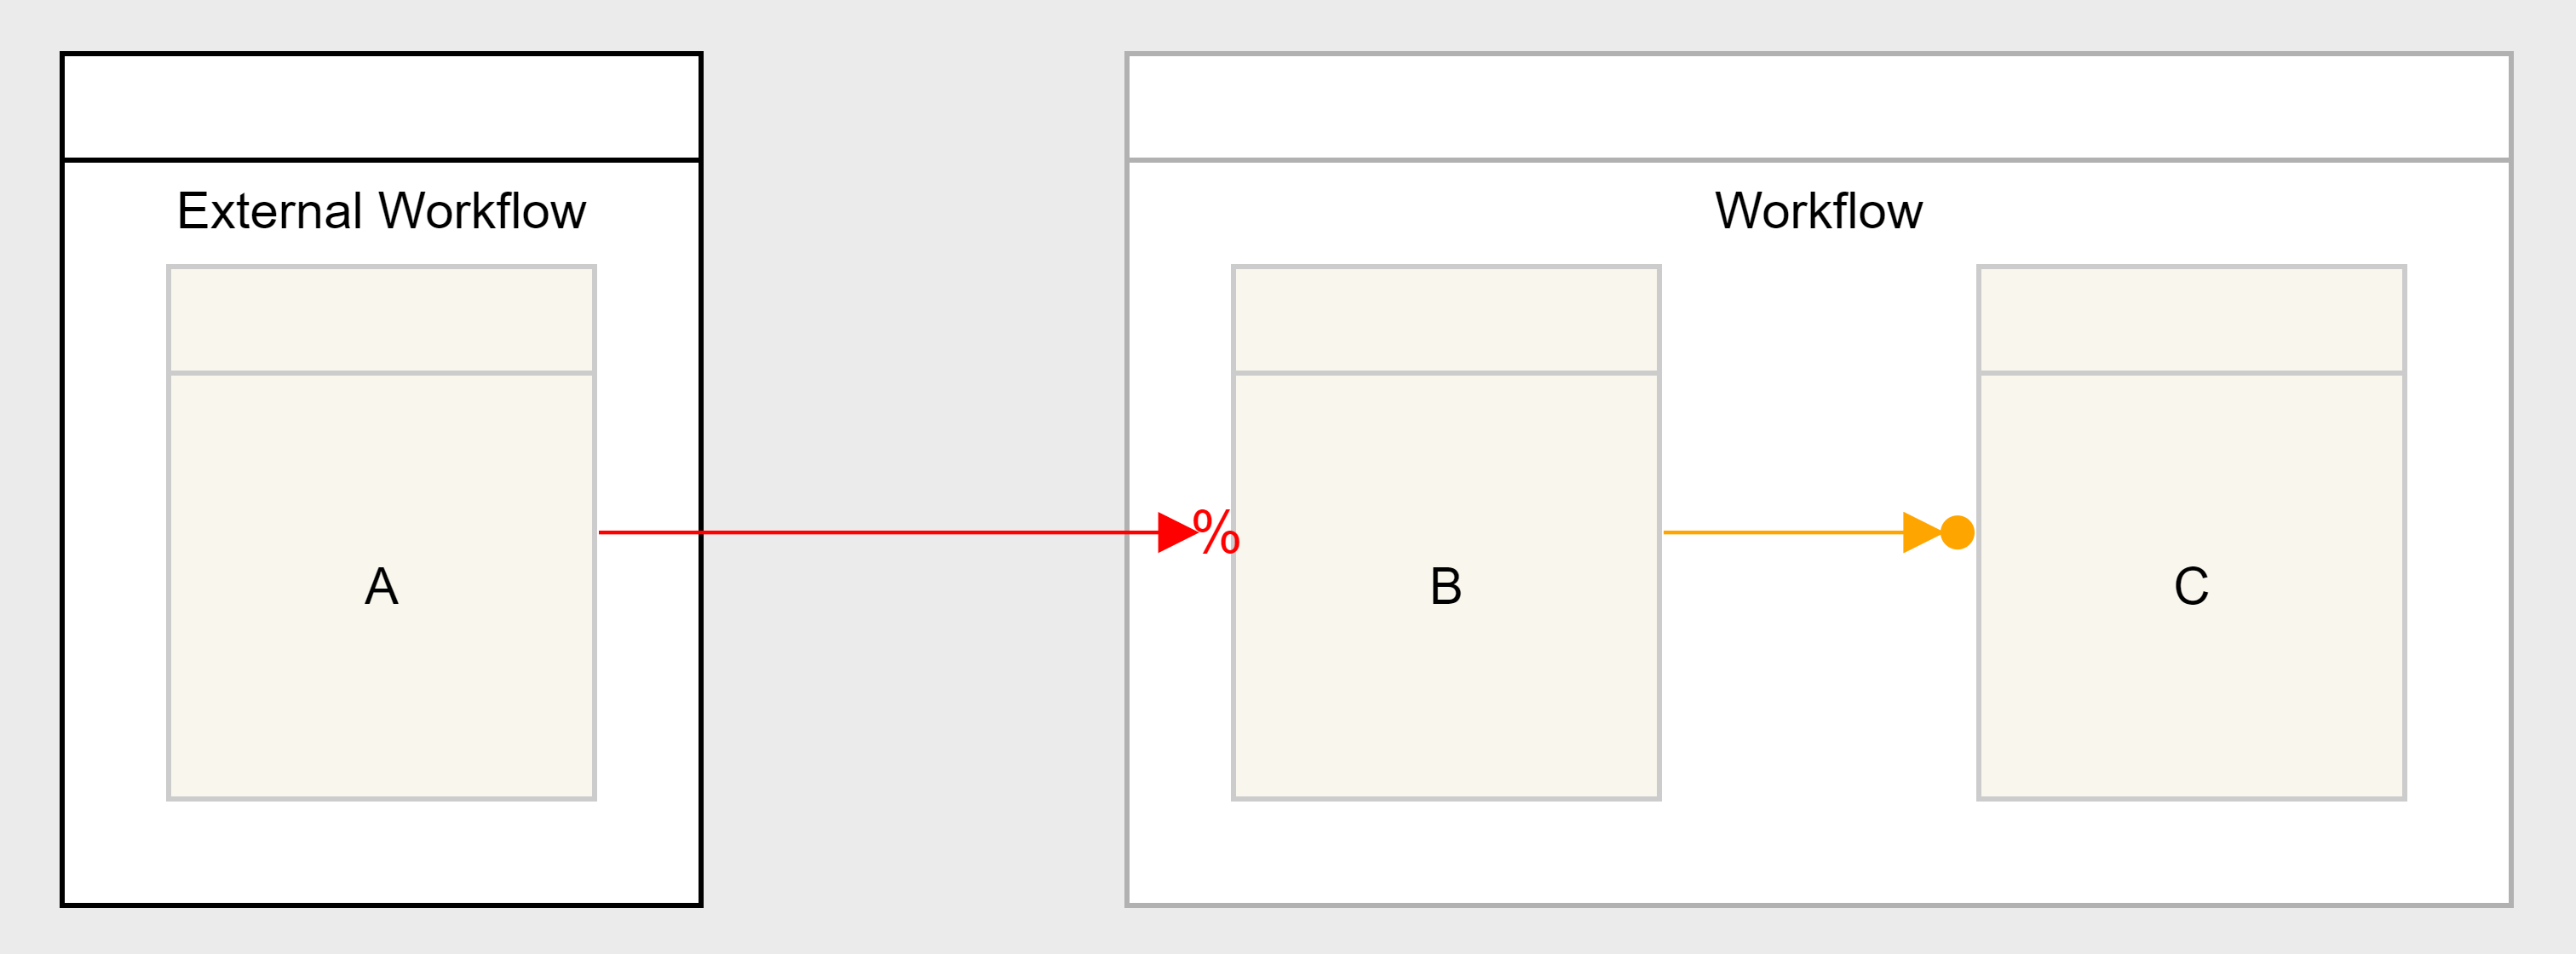
\includegraphics[scale=0.3]{figures/external-relations-example.png}
		 	\caption[External relation example]
		 	{External relation example. $A$ is a part of a different workflow than $B$ and $C$, but has an external exclude relation to $B$.}
		 	\label{fig:external-relations-example}
		\end{figure}


		But great care would be needed when allowing external workflows to create incoming relations to another workflow, as incoming relations can make workflows less restrictive, which is related to the issues outlined with regards to workflow changes (See section \ref{sec:workflow-changes}). 
		An example of this can be seen in figure \ref{fig:external-relations-example}, where $A$ in an external workflow has an exclude relation to an activity $B$ with a condition relation to another activity $C$ in the original workflow. 
		Executing $A$ would exclude $B$ and activity $C$ would be executable without executing $B$ as intended when constructing the condition relation.

		An implementation of this in the mono-contract solution would be fairly simple, as well as relatively cheap if the external workflow is stored in the same contract.

			\subsubsection{Vulnerabilities}
			Consider two workflows: $WF_{A}$ with activity $A$ and workflow $WF_{B}$ with activity $B$.
			If a relation $R$ from $A$ to $B$ is created, the resulting consequences depend greatly on whether or not the relation is an incoming relation or an outgoing relation.\footnote{See section \ref{sec:implementation-requirements}.}

			If $R$ is an outgoing relation, the representation of it will exist on $A$. 
			An execution of $A$ will propagate the changes of $R$ eagerly to $B$. 
			The execution of $A$ will therefore be more expensive.

			If $R$ is an incoming relation, the representation of it will exist on $B$. 
			An execution of $A$ will therefore be propagated lazily to $B$, as $B$ will not need to access the state of $A$ before a check if $B$ is executable is needed. 
			Checking if $B$ is in an executable state will be therefore be more expensive.

			Since an incoming relation from $A$ to $B$ both increases the cost of executing $A$ and propagates changes to $B$, the creator of $R$ must be the owner (or have equivalent rights) of $WF_{A}$ and $WF_{B}$.

			When $R$ is an outgoing relation from $A$ to $B$ the requirements are not as strict. $R$ will increase the cost of checking the executability of $B$, but no attribute of any activity in $A$ will be affected in any way. 
			Any external relation that conforms to the table below will therefore not result in any unwanted costs.

			\begin{table}[!ht]
				\begin{tabular}{|c|c|c|}
				\hline
				 					& Incoming 	& Outgoing \\ \hline
				$A \rightarrow B$ 	& Owns B    & Owns A+B \\
				\hline
				\end{tabular}
			\end{table}
			
			Needing ownership of both workflows is however quite restrictive.
			Another approach is to make the external outgoing relations lazy.
			This approach requires external relations to only be situated on the activity which changes state.
			Each time the activity containing the external relation is accessed, a check is made to determine the execution order of its dependencies.

			\begin{figure}[!ht]
				\centering
				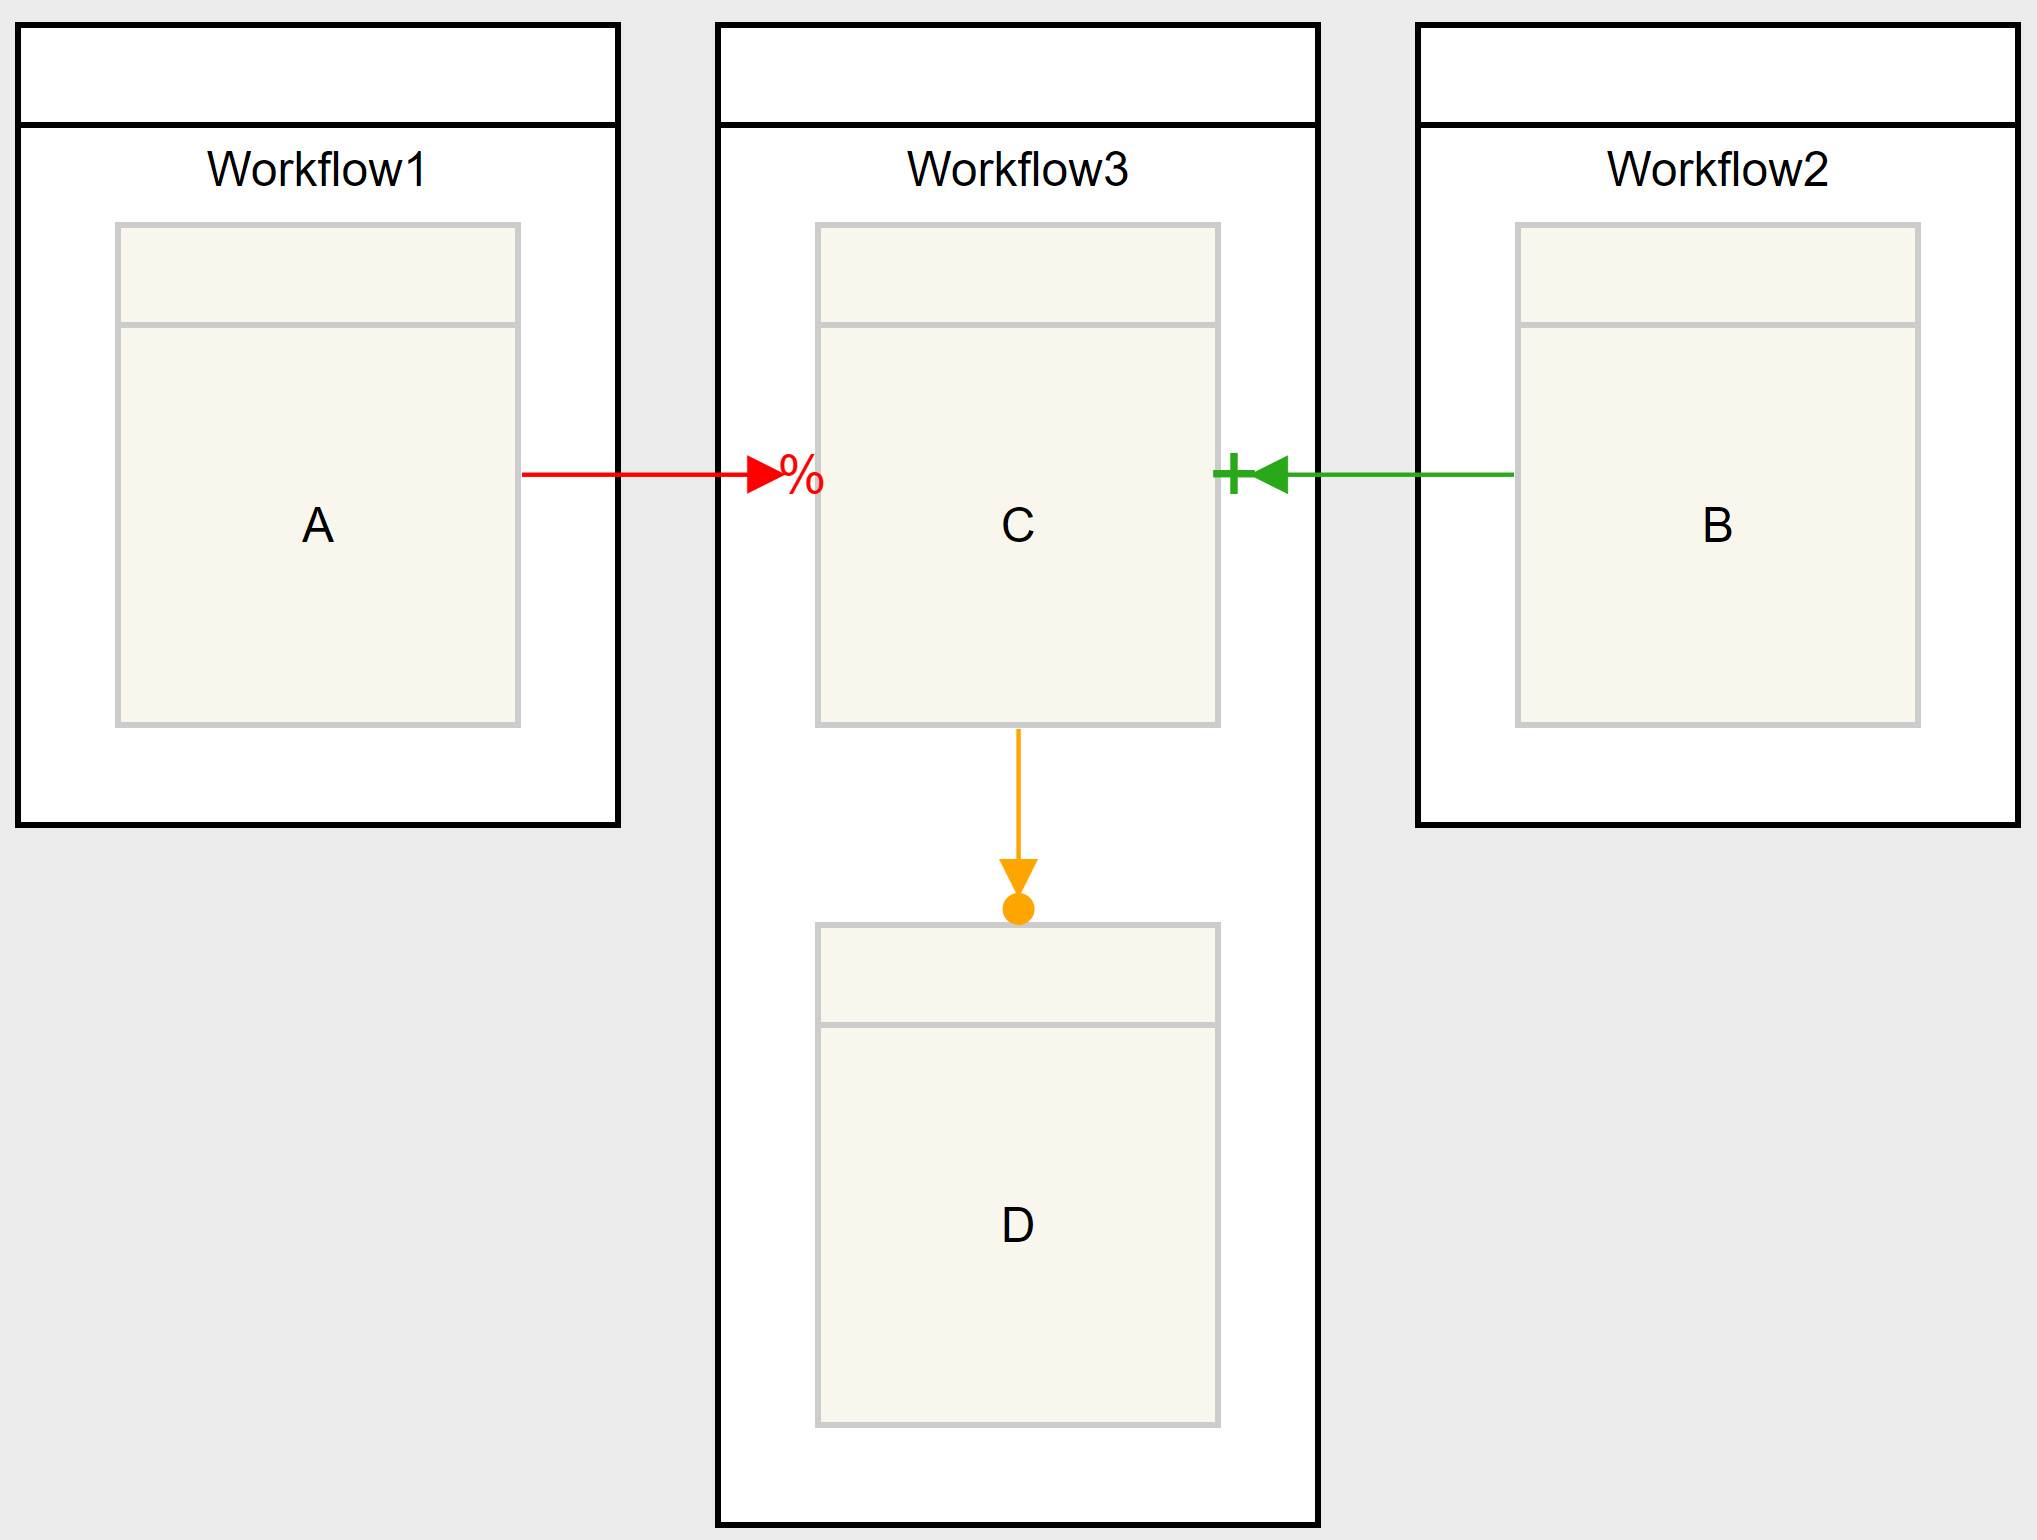
\includegraphics[scale=0.4]{figures/lazy-external-relation-example.PNG}
			 	\caption[Lazy external relation example]
			 	{Lazy external relation example. $\{A\}$, $\{B\}$ and $\{C, D\}$ are part of different workflows. The external relations to $C$ are only situated on $C$.}
			 	\label{fig:lazy-external-relations-example}
			\end{figure}

			However, this check is not trivial to design.
			Consider the situation in figure \ref{fig:lazy-external-relations-example}, where activities $A$ and $B$ are executed and both transactions containing the executions are collected in the same block. If the state of activity $C$ is accessed in a subsequent block, the state of $C$ cannot be determined without an absolute ordering of the executions.

			It is not possible for contracts to access previous states on the Ethereum blockchain, so the timestamps for the executions are not accessible, nor are the transaction hashes. 
			So an approach similar to that in \cite{bachelor}, where an absolute ordering is achieved by sorting on the hash, is not possible.
			Using logical clocks or vector clocks would also just conclude that the two executions are concurrent.
			We leave this problem open for further study.

		\subsection{External contract conditionals}
		As the public methods of a contract on the Ethereum blockchain are accessible by other contracts, provided they are called correctly and with sufficient funds, it would be possible to construct a workflow where some activities are dependent on the values of other contracts.
		These dependencies would essentially be conditional statements calling the functions of another contract, when it is being evaluated whether or not an activity is executable. 
		An example could be a contract returning the value of a currency and whether or not it is above or below a specified threshold.

		In the case where multiple companies have their own Mono-contract implementation, possibly due to their diverse needs for specific features, or the case where the Multi-contract implementation is used, this functionality would be closely tied to the functionality of external relations (See section \ref{sec:external-relations}).

			\subsubsection{Modeling external conditionals in DCR graphs}
			One could also incorporate DCR logic from external contracts, if a user creates a workflow with an activity where the only address authorized to execute the activity was the address of another contract.
			The external contract could either be created by the workflow creator, or it could be part of a service offered by external parties.
			The external party could be someone who monitored the price of certain commodities and executed the activity when certain criteria were met.
			
			Figure \ref{fig:external-contract-conditionals} shows how external contract conditionals can be implemented. 
			An external contract has been authorized to execute \texttt{Price of commodity above x} and \texttt{Price of commodity below x}. 
			Executing them will exclude or include \texttt{Price of commodity acceptable} which will allow or disallow execution of \texttt{Sell commodity}.
			
			In this example the activity \texttt{Price of commodity acceptable} is simply a placeholder activity and no user has the right to execute it.
			This can seem somewhat counterintuitive as activities usually are executable entities. 
			One could also place include and exclude relations from \texttt{Price of commodity above x} and \texttt{Price of commodity below x} directly to \texttt{Sell commodity}.
			This approach can however lead to complications if \texttt{Sell activity} has any condition relations to other activities as excluding \texttt{Sell activity} would allow execution of these activities.
			The first approach on the other hand preserves the restrictions of the original graph, and the external contract conditionals can therefore be added after workflow creation, if such a feature is supported in the particular DCR engine.
			Which approach is chosen is based on the intentions of the workflow creator.

			\begin{figure}[!ht]
				\centering
				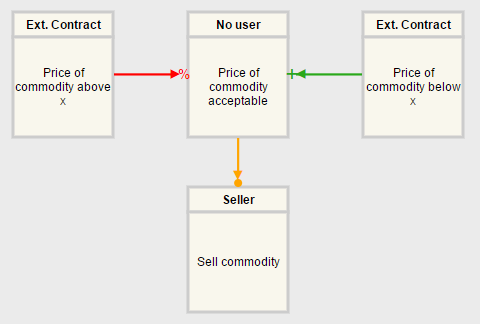
\includegraphics[scale=0.7]{figures/external-contract-conditionals.png}
			 	\caption[External contract conditionals]
			 	{Example of a DCR graph dependent on other contracts}
			 	\label{fig:external-contract-conditionals}
			\end{figure}

			\subsubsection{Vulnerabilities}

			If this feature would be implemented with actual calls to contracts, there are issues which need to be considered. 
			For example this was abused in the Decentralized Autonomous Organization (DAO) which existed on Ethereum.			
			The DAO was a venture capital fund, where the investors could vote on where to invest their collective money.
			It was one of the reasons for the growth of Ethereum and in May of 2016, they had attracted the users who owned 14\% of all Ether\cite{DAO}. 
			The investors had the option to withdraw their own funds, but an exploit was found in that the withdrawal finished by calling a given contract.
			This allowed a user to withdraw an amount of money and withdraw it again.
			This is not problematic in itself, but due to the balance only being updated as each method returns, a user was able to take 3.6 million Ether which was worth around 50 million dollars at the time.
			This exploit is called reentrancy and should be thoroughly investigated whenever external contract calls are allowed.

			In the case of DCR graphs, an external contract conditional could allow multiple executions when it shouldn't be possible, if the call is performed at the wrong time, as in this example:

			\begin{lstlisting}[language=pseudocode]
if (A.isIncluded)
	if (callContract) //External call
		...
			\end{lstlisting}

			The issue here is fairly anemic as it is not immediately apparent that this code is problematic.
			The issue is the potential side-effect of \emph{callContract}. 
			A potential side effect could be that the state of activity $A$ could have changed (it could be excluded) and its state therefore inconsistent with the intended state of it after the check to \emph{isIncluded}.
			The execution of activity $A$ would resume after \emph{callContract} and changes to other activities, if $A$ has outgoing relations, would be propagated even though $A$ would be excluded.  
			An external call should therefore be the very first thing called to ensure a consistent state and thereby avoid any reentrancy issues:

			\begin{lstlisting}[language=pseudocode]
if (callContract && A.included) //External call
	...
			\end{lstlisting}

		\subsection{Group authorization}
		A natural extension of the authorization mechanism would be to allow group authentication instead of only having a list of authorized users for each activity.
		This could prevent potential data duplication in cases where two or more users are authorized to execute exactly the same activities, which is a waste of storage on the blockchain.

		Group authorization could be implemented by storing the addresses of users that are part of a group in a list and then associating activities with the id of the group requiring execution rights.

		More specifically each user in a workflow should only need a single \emph{uint40}\footnote{We have chosen an \texttt{uint40} over a \texttt{uint32} to allow for eventual special groups such as authorization for workflow changes, deletion etc.} bitvector to support membership of 32 groups with individual authorizations. Each bit in the \emph{uint40} would indicate if a user was part of a group or not.

		Each activity in a workflow should then contain a \emph{uint32} where each bit represents whether or not a group has the rights to execute the activity.
		Lastly a workflow should contain a \emph{byte32} array of length 40 to store the group names.

		Even ignoring the optimizations this extension could bring, group authorization is still a valuable feature.
		The construction of workflows is much simpler without duplication of Ethereum-address and the transparency of how access rights are granted is improved.
		
	\section{Conclusion}

	\pagebreak
	\addcontentsline{toc}{section}{References}	
	\bibliographystyle{plain}
	\begin{thebibliography}{99}

		\bibitem{yellow-paper}
		Wood, G.
		\textit{Ethereum: A Secure Decentralised Generalised Transaction Ledger}. 
		\url{http://yellowpaper.io}.
		Accessed 2017-05-09.

		\bibitem{bachelor}
		Gaub et al.
		\textit{Consensus in peer-to-peer systems}.
		Unpublished manuscript.
		IT-University of Copenhagen,
		Denmark,
		2016.

		\bibitem{ethereum-white-paper}
		Various authors.
		\textit{White Paper}.
		\url{https://github.com/ethereum/wiki/wiki/White-Paper},
		Accessed 2017-05-09.

		\bibitem{bitcoin-white-paper}
		Nakamoto, S.
		\textit{Bitcoin: A Peer-to-Peer Electronic Cash System}.
		\url{https://bitcoin.org/bitcoin.pdf},
		Accessed 2017-05-09.

		\bibitem{distributed-workflows}
		Hildebrandt, T., Mukkamala, R. and Slaats, T.
		\textit{Safe Distribution of Declarative Processes}.
		\url{https://pure.itu.dk/ws/files/34548793/paper_5.pdf},
		Accessed 2017-05-10.

		\bibitem{hierarchical-declarative-modelling}
		Debois, S., Hildebrandt, T. and Slaats, T.
		\textit{Hierarchical Declarative Modelling with Refinement and Sub-processes}.
		\url{https://link.springer.com/chapter/10.1007%2F978-3-319-10172-9_2},
		Accessed 2017-05-11

		\bibitem{dynamic-workflows}
		Debois, S., Hildebrandt, T. and Slaats, T.
		\textit{HSafety, Liveness and Run-Time Refinement for Modular Process-Aware Information Systems with Dynamic Sub Processes}.
		\url{http://www.itu.dk/~debois/dcrstar-tr.pdf},
		Accessed 2017-05-12

		
		\bibitem{voting}
		Ethereum Foundation
		\textit{How to build a democracy on the blockchain}.
		\url{https://www.ethereum.org/dao},
		Accessed 2017-05-12

		\bibitem{anonymous-byzantine-consensus}
		LaViola Jr, JJ and Miller, A.
		\textit{Anonymous Byzantine Consensus from Moderately-Hard Puzzles: A Model for Bitcoin},
		2014

		\bibitem{DAO}
		Unknown author
		\textit{The DAO of accrue}.
		\url{https://www.economist.com/news/finance-and-economics/21699159-new-automated-investment-fund-has-attracted-stacks-digital-money-dao},
		Accessed 2017-05-13

		
		

	\end{thebibliography}

	\clearpage

	\addcontentsline{toc}{part}{Appendices}	

	\appendix

	\section{Gas prices}
		\label{app:gas-prices}

		As of May 9th, 2017, the gas prices are \cite{yellow-paper}: 
		\begin{table}[!ht]
		\footnotesize
		\noindent \begin{tabular}{| l | l | p{8cm} |}
			\hline
			Name 				& Value 	& Description \\ \hline
			$G_{zero}$ 			& 0 		& Nothing paid for operations of set $W_{zero}$. \\ \hline
			$G_{base}$ 			& 2 		& Amount of gas to pay for operations of the set $W_{base}$. \\ \hline
			$G_{verylow}$ 		& 3 		& Amount of gas to pay for operations of the set $W_{verylow}$. \\ \hline
			$G_{low}$ 			& 5 		& Amount of gas to pay for operations of the set $W_{low}$. \\ \hline
			$G_{mid}$ 			& 8 		& Amount of gas to pay for operations of the set $W_{mid}$. \\ \hline
			$G_{high}$ 			& 10 		& Amount of gas to pay for operations of the set $W_{high}$. \\ \hline
			$G_{extcode}$ 		& 700 		& Amount of gas to pay for operations of the set $W_{extcode}$. \\ \hline
			$G_{balance}$ 		& 400 		& Amount of gas to pay for a BALANCE operation. \\ \hline
			$G_{sload}$ 		& 200 		& Paid for a SLOAD operation. \\ \hline
			$G_{jumpdest}$ 		& 1 		& Paid for a JUMPDEST operation. \\ \hline
			$G_{sset}$ 			& 20000 	& Paid for an SSTORE operation when the storage value is set to non-zero from zero. \\ \hline
			$G_{sreset}$ 		& 5000 		& Paid for an SSTORE operation when the storage value's zeroness remains unchanged or is set to zero. \\ \hline
			$R_{sclear}$ 		& 15000		& Refund given (added into refund counter) when the storage value is set to zero from non-zero. \\ \hline
			$R_{suicide}$ 		& 24000 	& Refund given (added into refund counter) for suiciding an account. \\ \hline
			$G_{suicide}$ 		& 5000 		& Amount of gas to pay for a SUICIDE operation. \\ \hline
			$G_{create}$ 		& 32000		& Paid for a CREATE operation. \\ \hline
			$G_{codedeposit}$ 	& 200 		& Paid per byte for a CREATE operation to succeed in placing code into state. \\ \hline
			$G_{call}$ 			& 700		& Paid for a CALL operation. \\ \hline
			$G_{callvalue}$ 	& 9000		& Paid for a non-zero value transfer as part of the CALL operation. \\ \hline
			$G_{calstipend}$ 	& 2300		& A stipend for the called contract subtracted from $G_{callvalue}$ for a non-zero value transfer. \\ \hline
			$G_{newaccount}$ 	& 25000		& Paid for a CALL or SUICIDE operation which creates an account. \\ \hline
			$G_{exp}$ 			& 10 		& Partial payment for an EXP operation \\ \hline
			$G_{expbyte}$ 		& 10		& Partial payment when multiplied by $\ceil{log_{256}(exponent)}$  for the EXP operation. 	 \\ \hline
			$G_{memory}$ 		& 3			& Paid for every additional word when expanding memory. \\ \hline
			$G_{txcreate}$ 		& 32000		& Paid by all contract-creating transactions after the Homestead transition. \\ \hline
			$G_{txdatazero}$ 	& 4 		& Paid for every zero byte of data or code for a transaction. \\ \hline
			$G_{txdatanonzero}$ & 68		& Paid for every non-zero byte of data or code for a transaction. \\ \hline
			$G_{transaction}$ 	& 21000		& Paid for every transaction. \\ \hline
			$G_{log}$ 			& 375 		& Partial payment for a LOG operation. \\ \hline
			$G_{logdata}$ 		& 8			& Paid for each byte in a LOG operation's data. \\ \hline
			$G_{logtopic}$ 		& 375		& Paid for each topic of a LOG operation. \\ \hline
			$G_{sha3}$ 			& 30		& Paid for each SHA3 operation. \\ \hline
			$G_{sha3word}$ 		& 6			& Paid for each word (rounded up) for input data to a SHA3 operation. \\ \hline
			$G_{copy}$ 			& 3			& Partial payment for *COPY operations, multiplied by words copied, rounded up. \\ \hline
			$G_{blockhash}$ 	& 20		& Payment for BLOCKHASH operation. \\ 
			\hline
		\end{tabular}
		\end{table}
		\FloatBarrier

		\subsection{Instruction sets}
		\begin{description}
			\item[$W_{zero}$] = \{STOP, RETURN\}
			\item[$W_{base}$] = \{ADDRESS, ORIGIN, CALLER, CALLVALUE, CALLDATASIZE, CODESIZE, GASPRICE, COINBASE, TIMESTAMP, NUMBER, DIFFICULTY, GASLIMIT, POP, PC, MSIZE, GAS \}
			\item[$W_{verylow}$] = \{ADD, SUB, NOT, LT, GT, SLT, SGT, EQ, ISZERO, AND, OR, XOR, BYTE, CALLDATALOAD, MLOAD, MSTORE, MSTORES, PUSH*, DUP*, SWAP*\}
			\item[$W_{low}$] = \{MUL, DIV, SDIV, MOD, SMOD, SIGNEXTEND\}
			\item[$W_{mid}$] = \{ADDMOD, MULMOD, JUMP\}
			\item[$W_{high}$] = \{JUMPI\}
			\item[$W_{extcode}$] = \{EXTCODESIZE\}			
		\end{description}

	\section{Example workflow}
	\label{app:example-workflow}
		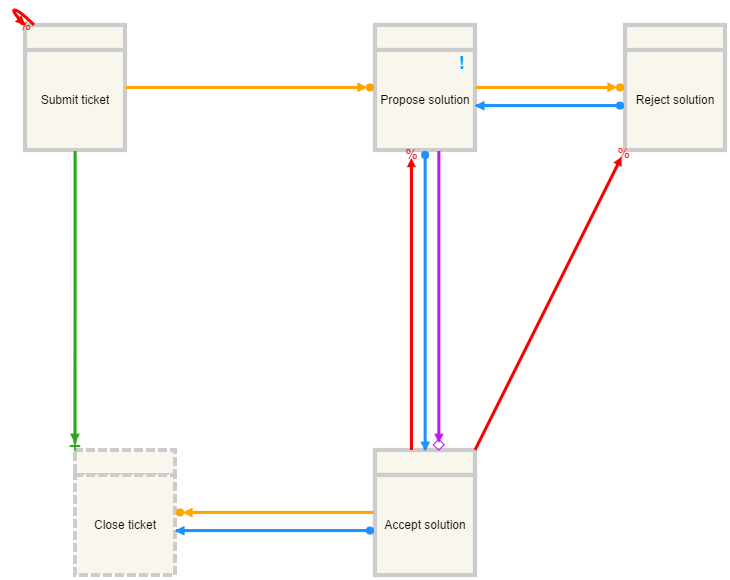
\includegraphics[scale=0.65, angle=90]{figures/ExampleWorkflow.png}
		\clearpage

	\section{Multi-contract code}
	\label{app:multi-contract-code}

		\lstinputlisting[language=solidity]{../contracts/workflow.sol}

	\section{Mono-contract code}

		\lstinputlisting[language=solidity]{../contracts/monolith.sol}

	\section{Mono-contract code with bitvectors}
		\label{app:mono-contract-code-with-bitvectors}


		\lstinputlisting[language=solidity]{../contracts/optimizations/monolith-bitvectors.sol}

	\pagebreak
	\section{Example workflow transaction hashes Multi-contract}
	\label{app:example-workflow-transaction-hashes-multi-contract}
		The table below shows the gas cost and transaction hashes (on the Ropsten testchain) for executions of the example workflow (see figure \ref{fig:exampleWorkflow}) in the multi-contract implementation.
		Since executions which throws an exception use all available gas in the transaction, the failing cases below have no meaningful gas cost. 
		However, they show that the execution behaves as expected.
		Also note that workflow creation is included in the cost of contract creation in the multi-contract implementation.
		\begin{longtable}{| l | p{0.12\textwidth} | p{0.5\textwidth} |}
			\hline 	
			Action 	 									& Gas cost 	  & TxHash on Ropsten Revived 													  \\\hline
			1. Contract creation						& 2221906 	  & \seqsplit{0x3f9a296d450ca9cdc4d73a7595add14f0c0b25421c8e34c5d087589b813a7734} \\\hline
			2. Workflow creation						& Included 
														in above cost & Included in transaction above \\\hline 
			3. Submit ticket (Authorization failure)	& - 		  & \seqsplit{0x6fe0bfe111b624b7ece7a64a1eeff6eed5ea7e9994794c5cb6462e9716568f99} \\\hline
			4. Propose solution (Condition failure)		& - 		  & \seqsplit{0xd3d39a1eb8539c6f9d2eadacb6c2114a4f3430141886372feac7359a33e334b8} \\\hline
			5. Reject solution (Condition failure)		& - 		  & \seqsplit{0xc598367828eb2ffd0fcafda581c501afed1f1da9139c745807338bc4a2a1277f} \\\hline
			6. Accept solution (Milestone failure)		& - 		  & \seqsplit{0x8cfc647a65a840d59c32776f9d856e08af089ae3a51a8342a51db5716f072ff4} \\\hline
			7. Close ticket (Excluded failure)			& - 		  & \seqsplit{0x21fa6c5c8458cdee8a546892001b01778639ca4e4855e53df83fa1e049c8d309} \\\hline
			8. Submit ticket							& 61112 	  & \seqsplit{0xb263f9e9f89a773ca1b4de65dc989e78e4cc9f939f13a161e27b8119e48a5cf4} \\\hline
			9. Submit ticket (Excluded failure)			& - 		  & \seqsplit{0xcfb70b00e0357a98eeabcca60d3bf9fba69d0f4724aa31c99df3542db0cfd988} \\\hline
			10. Propose solution						& 41208 	  & \seqsplit{0x923f1506887ea6d93ecea8c63e97e9e7d32d2227780d1c27764efbf8449b3bac} \\\hline
			11. Propose solution (Duplicate)			& 41208 	  & \seqsplit{0x7e361c81e441689408b1be3cf800be705b69228a30583b21d7fac40d61671147} \\\hline
			12. Reject solution							& 41208 	  & \seqsplit{0xff45cb12d828dccab36f96fcf2d18bffc85873fc0159afe392c506026dfe360c} \\\hline
			13. Propose solution						& 41208 	  & \seqsplit{0xd3373176d23c31cf1dc8e4314aec2d3d8012e5aff2edd4a57b56e278c6cf07b9} \\\hline
			14. Accept solution							& 54023 	  & \seqsplit{0xcff7205e63888de510e09c709f596d6dd65b559bba6a3f598a665c7f41ffcb60} \\\hline
			15. Close ticket							& 34810 	  & \seqsplit{0xbf0896427c4006153000cd5456d5ca23ba79f24da7242bb37b7746240d2038ce} \\\hline
		\end{longtable}

	\pagebreak
	\section{Example workflow transaction hashes Mono-contract}
	\label{app:example-workflow-transaction-hashes-mono-contract}
		The table below shows the gas cost and transaction hashes (on the Ropsten testchain) for executions of the example workflow (see figure \ref{fig:exampleWorkflow}) in the mono-contract implementation.
		Since executions which throws an exception use all available gas in the transaction, the failing cases below have no meaningful gas cost. 
		However, they show that the execution behaves as expected.
		Also note that the first workflow creation is more expensive that the two others, due to initializations of arrays. 
		\begin{longtable}{| l | p{0.12\textwidth} | p{0.5\textwidth} |}
			\hline 	
			Action 	 									& Gas cost 	& TxHash on Ropsten Revived 													\\\hline
			1. Contract creation						& 2183805	& \seqsplit{0x577ee5dd6c58747b983e4d6943ff6a14cbc380e630b0cbdca014a2837254e078} \\\hline
			2. Workflow creation (1)					& 1010934	& \seqsplit{0x12557a86b97721f87b471cbf1559e0dc8d0a1c6af2edb67b12cb796463a7cd92} \\\hline
			3. Submit ticket (Authorization failure) 	& -			& \seqsplit{0x301acf99c579ea0ed49099ff6c1e451fc9a5ef2e880c3292970e70c1af5cfcf9} \\\hline
			4. Propose solution (Condition failure)		& -			& \seqsplit{0x54fd86fb9388b6f2e5e89c83ff608f9fd81a48b08ff8d481e0bd41d4d2d78695} \\\hline
			5. Reject solution (Condition failure)		& -			& \seqsplit{0xe7d4485fb57cbeebc8a42107b4cd102e06ede6043e473fd99578d786ede469e5} \\\hline
			6. Accept solution (Milestone failure)		& -			& \seqsplit{0x2c097d5fdc31b0ffbb5ea424e8e1fc44af7addc89e4a707ba5f270ae9e650416} \\\hline
			7. Close ticket (Excluded failure)			& -			& \seqsplit{0xfaaad0773c564ad4913d55245f752871fabee7dca63bb3c93909e1a81e18bfb9} \\\hline
			8. Submit ticket							& 61187		& \seqsplit{0x95876f4c4a6652384c503593de0b609f3f7b41e28a9ae9eb6ee526241ff481e6} \\\hline
			9. Submit ticket (Excluded failure)			& -			& \seqsplit{0x81e047cd60aaa25ef3ef49c0a66bb74595aac4fd38e8bce809ff7c95bae0036c} \\\hline
			10. Propose solution						& 41263		& \seqsplit{0x5152469274c4f5f1958ee357640ebcb6b693118273b3defed26de3e58eff4cec} \\\hline
			11. Propose solution (Duplicate)			& 41263		& \seqsplit{0x6abcdff92de76d00d58afc9bb1816fb0c4da62077ec28a0bcf18dae1b0db3f63} \\\hline
			12. Reject solution							& 41263		& \seqsplit{0x662f8a264b1e4bea74d9e5255ff21b9395a23e72c120d6da7dc4bf798a820f59} \\\hline
			13. Propose solution						& 41263		& \seqsplit{0x9a021cd725465091372bc8ee7da4f17266cd829b57536bbcb8bdb8c08940070f} \\\hline
			14. Accept solution							& 54118		& \seqsplit{0x40e5e401f2b5bf46d64657df1695190460c560f56dacf0add8210c4db931c830} \\\hline
			15. Close ticket							& 34845		& \seqsplit{0x2f8b9c71252832f9975b1d95a7eb9f81090036fd2c4b54f42b6567cc96e1f6aa} \\\hline
			16. Workflow creation (2)					& 995934	& \seqsplit{0xe6b80f633324a9890a73c13542194d97048de1c326e3e23b5f2f6cc9b3f19ef6} \\\hline
			17. Workflow creation (3)					& 995934	& \seqsplit{0x860542d77bfc622cf4f97504876e4e4fbc8faaffa8189d6db1749ed43ec2762a} \\\hline
		\end{longtable}

	\pagebreak
	\section{Test cases gas comparison for example workflow}
	\label{app:test-cases-gas}
		The table below brings together the gas costs from appendencies \ref{app:example-workflow-transaction-hashes-multi-contract} and \ref{app:example-workflow-transaction-hashes-mono-contract} for gas cost comparison.

		\begin{tabular}{| l | l | l |}
			\hline
			Action 										& Multi-contract & Mono-contract \\ \hline
			1. Contract creation						& 2221906		 & 2183805 	\\\hline
			2. Workflow creation						& included 		 & 1010934 	\\\hline
			3. Submit ticket (Authorization failure)	& -				 & - 		\\\hline
			4. Propose solution (Condition failure)		& -				 & - 		\\\hline
			5. Reject solution (Condition failure)		& -				 & - 		\\\hline
			6. Accept solution (Milestone failure)		& -				 & - 		\\\hline
			7. Close ticket (Excluded failure)			& -				 & - 		\\\hline
			8. Submit ticket							& 61112			 & 61187 	\\\hline
			9. Submit ticket (Excluded failure)			& -				 & - 		\\\hline
			10. Propose solution						& 41208			 & 41263 	\\\hline
			11. Propose solution (Duplicate)			& 41208			 & 41263 	\\\hline
			12. Reject solution							& 41208			 & 41263 	\\\hline
			13. Propose solution						& 41208			 & 41263 	\\\hline
			14. Accept solution							& 54023			 & 54118 	\\\hline
			15. Close ticket							& 34810			 & 34845 	\\\hline
			16. Workflow creation (2)					& -				 & 995934 	\\\hline
			17. Workflow creation (3)					& -				 & 995934 	\\\hline
			\hline
		\end{tabular}

		\pagebreak

	\section{Example workflow transaction hashes Mono-contract with bitvectors}
	\label{app:example-workflow-transaction-hashes-mono-contract-with-bitvectors}
		\begin{longtable}{| l | p{0.12\textwidth} | p{0.5\textwidth} |}
			\hline 	
			Action 	 						& Gas cost 	& TxHash on Ropsten Revived 													\\\hline
			1. Contract creation			& 1708991	& \seqsplit{0xcd5133cef32d5a41f2830fdc85b227fa3e33c930e258599f59aa012dd59c4d92} \\\hline
			2. Workflow creation (1)		& 835045	& \seqsplit{0x4134e6eca1af2caf030519ff0c2aad02e6787925b1fe9f1e9a14f8f795ae1fbb} \\\hline
			3. Submit ticket				& 66591		& \seqsplit{0xc109656addb462e09b8167a2e01858c42b97fc484b153b1aed2a503aca3ae112} \\\hline
			4. Propose solution				& 51805		& \seqsplit{0xd7a69bc9d835c8a696d0df1a77575a151c4da49fcf3811a4aec20d1259de2898} \\\hline
			5. Propose solution (Duplicate)	& 51805		& \seqsplit{0x38afda857b8f5bd59cef819d98440473a2336926cf95765559bd236cd06085c4} \\\hline
			6. Reject solution				& 51805		& \seqsplit{0x84e8270c23b4ba2a46fc98aa841970ace36c53fdc01e999f2d5ac48a30a65c34} \\\hline
			7. Propose solution				& 51805		& \seqsplit{0xb868f7f9c96d248c9694fdcd7e721c72d417e68258dfd67a86a0f4f6c27d9ce4} \\\hline
			8. Accept solution				& 51805		& \seqsplit{0xfb47b6c2d207ac9bba7eede93710af908ce70b9f245dab87a11af66ba0ee253e} \\\hline
			9. Close ticket					& 36805		& \seqsplit{0x1b84e19e2ca5270174546fbaacd97fb17240588d4bf0b6235fabe4ccd2311388} \\\hline
			10.Workflow creation (2)		& 820045	& \seqsplit{0x497a26e6615a4262e25eadee29dbd5bd1f7e8f763255a4940ad574052d41ca5c} \\\hline
			11.Workflow creation (3)		& 820045	& \seqsplit{0x44b86c4630a260cc7038b42aa63961474992bd1bee97186de7b70543c5c99775} \\\hline
		\end{longtable}

	\section{Test cases gas comparison for example workflow}
	\label{app:test-cases-gas}
		The table below brings together the gas costs from appendencies \ref{app:example-workflow-transaction-hashes-multi-contract} and \ref{app:example-workflow-transaction-hashes-mono-contract} for gas cost comparison.

		\begin{tabular}{| l | l | l |}
			\hline
			Action 							& Mono-contract  & Mono-contract with bitvectors \\ \hline
			1. Contract creation			& 2183805		 & 1708991 	\\\hline
			2. Workflow creation (1)		& 1010934 		 & 835045 	\\\hline
			3. Submit ticket				& 61187			 & 66591	\\\hline
			4. Propose solution				& 41263 		 & 51805	\\\hline
			5. Propose solution (Duplicate)	& 41263 		 & 51805	\\\hline
			6. Reject solution				& 41263 		 & 51805	\\\hline
			7. Propose solution				& 41263 		 & 51805	\\\hline
			8. Accept solution				& 54118 		 & 51805	\\\hline
			9. Close ticket					& 34845 		 & 36805	\\\hline
			10.Workflow creation (2)		& 995934 		 & 820045	\\\hline
			11.Workflow creation (3)		& 995934 		 & 820045	\\\hline
			\hline
		\end{tabular}
		\pagebreak


% \pagebreak
	% \section{Edge and stress test workflow transaction hashes Multi-contract}
	% \label{app:edge-and-stress-test-workflow-hashes-multi-contract}
	% 	The table below shows the gas cost and transaction hashes (on the Ropsten testchain) for executions of the example workflow (see figure \ref{fig:exampleWorkflow}) in the multi-contract implementation.
	% 	Since executions which throws an exception use all available gas in the transaction, the failing cases below have no meaningful gas cost. 
	% 	However, they show that the execution behaves as expected.
	% 	Also note that workflow creation is included in the cost of contract creation in the multi-contract implementation.
	% 	\begin{longtable}{| l | p{0.12\textwidth} | p{0.5\textwidth} |}
	% 		\hline 	
	% 		Action 	 									& Gas cost 	  & TxHash on Ropsten Revived 													  \\\hline
	% 		1. Contract creation						& 2221906 	  & \seqsplit{0x3f9a296d450ca9cdc4d73a7595add14f0c0b25421c8e34c5d087589b813a7734} \\\hline
	% 		2. Workflow creation						& Included 
	% 													in above cost & Included in transaction above \\\hline 
	% 		3. Submit ticket (Authorization failure)	& - 		  & \seqsplit{0x6fe0bfe111b624b7ece7a64a1eeff6eed5ea7e9994794c5cb6462e9716568f99} \\\hline
	% 		4. Propose solution (Condition failure)		& - 		  & \seqsplit{0xd3d39a1eb8539c6f9d2eadacb6c2114a4f3430141886372feac7359a33e334b8} \\\hline
	% 		5. Reject solution (Condition failure)		& - 		  & \seqsplit{0xc598367828eb2ffd0fcafda581c501afed1f1da9139c745807338bc4a2a1277f} \\\hline
	% 		6. Accept solution (Milestone failure)		& - 		  & \seqsplit{0x8cfc647a65a840d59c32776f9d856e08af089ae3a51a8342a51db5716f072ff4} \\\hline
	% 		7. Close ticket (Excluded failure)			& - 		  & \seqsplit{0x21fa6c5c8458cdee8a546892001b01778639ca4e4855e53df83fa1e049c8d309} \\\hline
	% 		8. Submit ticket							& 61112 	  & \seqsplit{0xb263f9e9f89a773ca1b4de65dc989e78e4cc9f939f13a161e27b8119e48a5cf4} \\\hline
	% 		9. Submit ticket (Excluded failure)			& - 		  & \seqsplit{0xcfb70b00e0357a98eeabcca60d3bf9fba69d0f4724aa31c99df3542db0cfd988} \\\hline
	% 		10. Propose solution						& 41208 	  & \seqsplit{0x923f1506887ea6d93ecea8c63e97e9e7d32d2227780d1c27764efbf8449b3bac} \\\hline
	% 		11. Propose solution (Duplicate)			& 41208 	  & \seqsplit{0x7e361c81e441689408b1be3cf800be705b69228a30583b21d7fac40d61671147} \\\hline
	% 		12. Reject solution							& 41208 	  & \seqsplit{0xff45cb12d828dccab36f96fcf2d18bffc85873fc0159afe392c506026dfe360c} \\\hline
	% 		13. Propose solution						& 41208 	  & \seqsplit{0xd3373176d23c31cf1dc8e4314aec2d3d8012e5aff2edd4a57b56e278c6cf07b9} \\\hline
	% 		14. Accept solution							& 54023 	  & \seqsplit{0xcff7205e63888de510e09c709f596d6dd65b559bba6a3f598a665c7f41ffcb60} \\\hline
	% 		15. Close ticket							& 34810 	  & \seqsplit{0xbf0896427c4006153000cd5456d5ca23ba79f24da7242bb37b7746240d2038ce} \\\hline
	% 	\end{longtable}

	% \pagebreak
	% \section{Edge and stress test workflow transaction hashes Mono-contract}
	% \label{app:edge-and-stress-test-workflow-hashes-mono-contract}
	% 	The table below shows the gas cost and transaction hashes (on the Ropsten testchain) for executions of the example workflow (see figure \ref{fig:exampleWorkflow}) in the mono-contract implementation.
	% 	Since executions which throws an exception use all available gas in the transaction, the failing cases below have no meaningful gas cost. 
	% 	However, they show that the execution behaves as expected.
	% 	Also note that the first workflow creation is more expensive that the two others, due to initializations of arrays. 
	% 	\begin{longtable}{| l | p{0.12\textwidth} | p{0.5\textwidth} |}
	% 		\hline 	
	% 		Action 	 									& Gas cost 	& TxHash on Ropsten Revived 													\\\hline
	% 		1. Contract creation						& 2183805	& \seqsplit{0x577ee5dd6c58747b983e4d6943ff6a14cbc380e630b0cbdca014a2837254e078} \\\hline
	% 		2. Workflow creation (1)					& 1010934	& \seqsplit{0x12557a86b97721f87b471cbf1559e0dc8d0a1c6af2edb67b12cb796463a7cd92} \\\hline
	% 		3. Submit ticket (Authorization failure) 	& -			& \seqsplit{0x301acf99c579ea0ed49099ff6c1e451fc9a5ef2e880c3292970e70c1af5cfcf9} \\\hline
	% 		4. Propose solution (Condition failure)		& -			& \seqsplit{0x54fd86fb9388b6f2e5e89c83ff608f9fd81a48b08ff8d481e0bd41d4d2d78695} \\\hline
	% 		5. Reject solution (Condition failure)		& -			& \seqsplit{0xe7d4485fb57cbeebc8a42107b4cd102e06ede6043e473fd99578d786ede469e5} \\\hline
	% 		6. Accept solution (Milestone failure)		& -			& \seqsplit{0x2c097d5fdc31b0ffbb5ea424e8e1fc44af7addc89e4a707ba5f270ae9e650416} \\\hline
	% 		7. Close ticket (Excluded failure)			& -			& \seqsplit{0xfaaad0773c564ad4913d55245f752871fabee7dca63bb3c93909e1a81e18bfb9} \\\hline
	% 		8. Submit ticket							& 61187		& \seqsplit{0x95876f4c4a6652384c503593de0b609f3f7b41e28a9ae9eb6ee526241ff481e6} \\\hline
	% 		9. Submit ticket (Excluded failure)			& -			& \seqsplit{0x81e047cd60aaa25ef3ef49c0a66bb74595aac4fd38e8bce809ff7c95bae0036c} \\\hline
	% 		10. Propose solution						& 41263		& \seqsplit{0x5152469274c4f5f1958ee357640ebcb6b693118273b3defed26de3e58eff4cec} \\\hline
	% 		11. Propose solution (Duplicate)			& 41263		& \seqsplit{0x6abcdff92de76d00d58afc9bb1816fb0c4da62077ec28a0bcf18dae1b0db3f63} \\\hline
	% 		12. Reject solution							& 41263		& \seqsplit{0x662f8a264b1e4bea74d9e5255ff21b9395a23e72c120d6da7dc4bf798a820f59} \\\hline
	% 		13. Propose solution						& 41263		& \seqsplit{0x9a021cd725465091372bc8ee7da4f17266cd829b57536bbcb8bdb8c08940070f} \\\hline
	% 		14. Accept solution							& 54118		& \seqsplit{0x40e5e401f2b5bf46d64657df1695190460c560f56dacf0add8210c4db931c830} \\\hline
	% 		15. Close ticket							& 34845		& \seqsplit{0x2f8b9c71252832f9975b1d95a7eb9f81090036fd2c4b54f42b6567cc96e1f6aa} \\\hline
	% 		16. Workflow creation (2)					& 995934	& \seqsplit{0xe6b80f633324a9890a73c13542194d97048de1c326e3e23b5f2f6cc9b3f19ef6} \\\hline
	% 		17. Workflow creation (3)					& 995934	& \seqsplit{0x860542d77bfc622cf4f97504876e4e4fbc8faaffa8189d6db1749ed43ec2762a} \\\hline
	% 	\end{longtable}
	% \pagebreak
	% \section{Test cases gas comparison for example workflow}
	% \label{app:test-cases-gas}

	% 	\begin{tabular}{| l | l | l |}
	% 		\hline
	% 		Action 										& Multi-contract & Mono-contract \\ \hline
	% 		1. Contract creation						& 2221906		 & 2183805 	\\\hline
	% 		2. Workflow creation						& included 		 & 1010934 	\\\hline
	% 		3. Submit ticket (Authorization failure)	& -				 & - 		\\\hline
	% 		4. Propose solution (Condition failure)		& -				 & - 		\\\hline
	% 		5. Reject solution (Condition failure)		& -				 & - 		\\\hline
	% 		6. Accept solution (Milestone failure)		& -				 & - 		\\\hline
	% 		7. Close ticket (Excluded failure)			& -				 & - 		\\\hline
	% 		8. Submit ticket							& 61112			 & 61187 	\\\hline
	% 		9. Submit ticket (Excluded failure)			& -				 & - 		\\\hline
	% 		10. Propose solution						& 41208			 & 41263 	\\\hline
	% 		11. Propose solution (Duplicate)			& 41208			 & 41263 	\\\hline
	% 		12. Reject solution							& 41208			 & 41263 	\\\hline
	% 		13. Propose solution						& 41208			 & 41263 	\\\hline
	% 		14. Accept solution							& 54023			 & 54118 	\\\hline
	% 		15. Close ticket							& 34810			 & 34845 	\\\hline
	% 		16. Workflow creation (2)					& -				 & 995934 	\\\hline
	% 		17. Workflow creation (3)					& -				 & 995934 	\\\hline
	% 		\hline
	% 	\end{tabular}

	% \section{Stress and edge tests}
	% \label{app:stress-and-edge-tests}

	% 	\begin{tabular}{| l | l | l |}
	% 		\hline
	% 		Test & Multi-contract & Mono-contract \\ \hline
	% 		C1.1 & 0 & 0 \\ \hline
	% 		M1.1 & 0 & 0 \\ \hline
	% 		C2.1 & 0 & 0 \\ \hline
	% 		M2.1 & 0 & 0 \\ \hline
	% 		I1.1 & 0 & 0 \\ \hline
	% 		E1.1 & 0 & 0 \\ \hline
	% 		R1.1 & 0 & 0 \\ \hline
	% 		I2.1 & 0 & 0 \\ \hline
	% 		E2.1 & 0 & 0 \\ \hline
	% 		R2.1 & 0 & 0 \\ \hline
	% 		C-stress1 & 0 & 0 \\ \hline
	% 		C-stress2 & 0 & 0 \\ \hline
	% 		M-stress1 & 0 & 0 \\ \hline
	% 		M-stress2 & 0 & 0 \\ \hline
	% 		P-stress1 & 0 & 0 \\ \hline
	% 		I-stress1 & 0 & 0 \\
	% 		\hline
	% 	\end{tabular}

\end{document}